% Options for packages loaded elsewhere
\PassOptionsToPackage{unicode}{hyperref}
\PassOptionsToPackage{hyphens}{url}
%
\documentclass[
]{book}
\title{R과 통계분석}
\author{박동련}
\date{2022-02-11}

\usepackage{amsmath,amssymb}
\usepackage{lmodern}
\usepackage{iftex}
\ifPDFTeX
  \usepackage[T1]{fontenc}
  \usepackage[utf8]{inputenc}
  \usepackage{textcomp} % provide euro and other symbols
\else % if luatex or xetex
  \usepackage{unicode-math}
  \defaultfontfeatures{Scale=MatchLowercase}
  \defaultfontfeatures[\rmfamily]{Ligatures=TeX,Scale=1}
\fi
% Use upquote if available, for straight quotes in verbatim environments
\IfFileExists{upquote.sty}{\usepackage{upquote}}{}
\IfFileExists{microtype.sty}{% use microtype if available
  \usepackage[]{microtype}
  \UseMicrotypeSet[protrusion]{basicmath} % disable protrusion for tt fonts
}{}
\makeatletter
\@ifundefined{KOMAClassName}{% if non-KOMA class
  \IfFileExists{parskip.sty}{%
    \usepackage{parskip}
  }{% else
    \setlength{\parindent}{0pt}
    \setlength{\parskip}{6pt plus 2pt minus 1pt}}
}{% if KOMA class
  \KOMAoptions{parskip=half}}
\makeatother
\usepackage{xcolor}
\IfFileExists{xurl.sty}{\usepackage{xurl}}{} % add URL line breaks if available
\IfFileExists{bookmark.sty}{\usepackage{bookmark}}{\usepackage{hyperref}}
\hypersetup{
  pdftitle={R과 통계분석},
  pdfauthor={박동련},
  hidelinks,
  pdfcreator={LaTeX via pandoc}}
\urlstyle{same} % disable monospaced font for URLs
\usepackage{color}
\usepackage{fancyvrb}
\newcommand{\VerbBar}{|}
\newcommand{\VERB}{\Verb[commandchars=\\\{\}]}
\DefineVerbatimEnvironment{Highlighting}{Verbatim}{commandchars=\\\{\}}
% Add ',fontsize=\small' for more characters per line
\usepackage{framed}
\definecolor{shadecolor}{RGB}{248,248,248}
\newenvironment{Shaded}{\begin{snugshade}}{\end{snugshade}}
\newcommand{\AlertTok}[1]{\textcolor[rgb]{0.94,0.16,0.16}{#1}}
\newcommand{\AnnotationTok}[1]{\textcolor[rgb]{0.56,0.35,0.01}{\textbf{\textit{#1}}}}
\newcommand{\AttributeTok}[1]{\textcolor[rgb]{0.77,0.63,0.00}{#1}}
\newcommand{\BaseNTok}[1]{\textcolor[rgb]{0.00,0.00,0.81}{#1}}
\newcommand{\BuiltInTok}[1]{#1}
\newcommand{\CharTok}[1]{\textcolor[rgb]{0.31,0.60,0.02}{#1}}
\newcommand{\CommentTok}[1]{\textcolor[rgb]{0.56,0.35,0.01}{\textit{#1}}}
\newcommand{\CommentVarTok}[1]{\textcolor[rgb]{0.56,0.35,0.01}{\textbf{\textit{#1}}}}
\newcommand{\ConstantTok}[1]{\textcolor[rgb]{0.00,0.00,0.00}{#1}}
\newcommand{\ControlFlowTok}[1]{\textcolor[rgb]{0.13,0.29,0.53}{\textbf{#1}}}
\newcommand{\DataTypeTok}[1]{\textcolor[rgb]{0.13,0.29,0.53}{#1}}
\newcommand{\DecValTok}[1]{\textcolor[rgb]{0.00,0.00,0.81}{#1}}
\newcommand{\DocumentationTok}[1]{\textcolor[rgb]{0.56,0.35,0.01}{\textbf{\textit{#1}}}}
\newcommand{\ErrorTok}[1]{\textcolor[rgb]{0.64,0.00,0.00}{\textbf{#1}}}
\newcommand{\ExtensionTok}[1]{#1}
\newcommand{\FloatTok}[1]{\textcolor[rgb]{0.00,0.00,0.81}{#1}}
\newcommand{\FunctionTok}[1]{\textcolor[rgb]{0.00,0.00,0.00}{#1}}
\newcommand{\ImportTok}[1]{#1}
\newcommand{\InformationTok}[1]{\textcolor[rgb]{0.56,0.35,0.01}{\textbf{\textit{#1}}}}
\newcommand{\KeywordTok}[1]{\textcolor[rgb]{0.13,0.29,0.53}{\textbf{#1}}}
\newcommand{\NormalTok}[1]{#1}
\newcommand{\OperatorTok}[1]{\textcolor[rgb]{0.81,0.36,0.00}{\textbf{#1}}}
\newcommand{\OtherTok}[1]{\textcolor[rgb]{0.56,0.35,0.01}{#1}}
\newcommand{\PreprocessorTok}[1]{\textcolor[rgb]{0.56,0.35,0.01}{\textit{#1}}}
\newcommand{\RegionMarkerTok}[1]{#1}
\newcommand{\SpecialCharTok}[1]{\textcolor[rgb]{0.00,0.00,0.00}{#1}}
\newcommand{\SpecialStringTok}[1]{\textcolor[rgb]{0.31,0.60,0.02}{#1}}
\newcommand{\StringTok}[1]{\textcolor[rgb]{0.31,0.60,0.02}{#1}}
\newcommand{\VariableTok}[1]{\textcolor[rgb]{0.00,0.00,0.00}{#1}}
\newcommand{\VerbatimStringTok}[1]{\textcolor[rgb]{0.31,0.60,0.02}{#1}}
\newcommand{\WarningTok}[1]{\textcolor[rgb]{0.56,0.35,0.01}{\textbf{\textit{#1}}}}
\usepackage{longtable,booktabs,array}
\usepackage{calc} % for calculating minipage widths
% Correct order of tables after \paragraph or \subparagraph
\usepackage{etoolbox}
\makeatletter
\patchcmd\longtable{\par}{\if@noskipsec\mbox{}\fi\par}{}{}
\makeatother
% Allow footnotes in longtable head/foot
\IfFileExists{footnotehyper.sty}{\usepackage{footnotehyper}}{\usepackage{footnote}}
\makesavenoteenv{longtable}
\usepackage{graphicx}
\makeatletter
\def\maxwidth{\ifdim\Gin@nat@width>\linewidth\linewidth\else\Gin@nat@width\fi}
\def\maxheight{\ifdim\Gin@nat@height>\textheight\textheight\else\Gin@nat@height\fi}
\makeatother
% Scale images if necessary, so that they will not overflow the page
% margins by default, and it is still possible to overwrite the defaults
% using explicit options in \includegraphics[width, height, ...]{}
\setkeys{Gin}{width=\maxwidth,height=\maxheight,keepaspectratio}
% Set default figure placement to htbp
\makeatletter
\def\fps@figure{htbp}
\makeatother
\setlength{\emergencystretch}{3em} % prevent overfull lines
\providecommand{\tightlist}{%
  \setlength{\itemsep}{0pt}\setlength{\parskip}{0pt}}
\setcounter{secnumdepth}{5}
\usepackage{booktabs}
\ifLuaTeX
  \usepackage{selnolig}  % disable illegal ligatures
\fi
\usepackage[]{natbib}
\bibliographystyle{plainnat}

\begin{document}
\maketitle

{
\setcounter{tocdepth}{1}
\tableofcontents
}
\hypertarget{uxc18cuxac1cuxd558uxae30}{%
\chapter*{소개하기}\label{uxc18cuxac1cuxd558uxae30}}
\addcontentsline{toc}{chapter}{소개하기}


\includegraphics{Figure/cover.jpg}

\hypertarget{r-uxc2dcuxc791uxd558uxae30}{%
\chapter{R 시작하기}\label{r-uxc2dcuxc791uxd558uxae30}}

Placeholder

\hypertarget{ruxc758-uxc18cuxac1c}{%
\section{R의 소개}\label{ruxc758-uxc18cuxac1c}}

\hypertarget{ruxc758-uxc124uxce58}{%
\section{R의 설치}\label{ruxc758-uxc124uxce58}}

\hypertarget{rstudiouxc758-uxc124uxce58-uxbc0f-ruxc758-uxc2e4uxd589}{%
\section{RStudio의 설치 및 R의 실행}\label{rstudiouxc758-uxc124uxce58-uxbc0f-ruxc758-uxc2e4uxd589}}

\hypertarget{uxc791uxc5c5uxacf5uxac04}{%
\section{작업공간}\label{uxc791uxc5c5uxacf5uxac04}}

\hypertarget{uxc2a4uxd06cuxb9bduxd2b8-uxd30cuxc77cuxc758-uxd65cuxc6a9}{%
\section{스크립트 파일의 활용}\label{uxc2a4uxd06cuxb9bduxd2b8-uxd30cuxc77cuxc758-uxd65cuxc6a9}}

\hypertarget{section-batch}{%
\section{일괄처리}\label{section-batch}}

\hypertarget{section-package}{%
\section{R의 확장: 패키지}\label{section-package}}

\hypertarget{uxd328uxd0a4uxc9c0uxc758-uxc885uxb958}{%
\subsection{패키지의 종류}\label{uxd328uxd0a4uxc9c0uxc758-uxc885uxb958}}

\hypertarget{uxd328uxd0a4uxc9c0uxc758-uxc124uxce58-uxbc0f-uxc0acuxc6a9}{%
\subsection{패키지의 설치 및 사용}\label{uxd328uxd0a4uxc9c0uxc758-uxc124uxce58-uxbc0f-uxc0acuxc6a9}}

\hypertarget{uxd328uxd0a4uxc9c0-tidyverseuxc758-uxc18cuxac1c}{%
\subsection{패키지 tidyverse의 소개}\label{uxd328uxd0a4uxc9c0-tidyverseuxc758-uxc18cuxac1c}}

\hypertarget{data-structure}{%
\chapter{R 데이터 구조}\label{data-structure}}

통계학에서 데이터는 양적 데이터와 질적 데이터로 구분된다.
양적 데이터는 숫자형 데이터를 의미하는 것으로서 연속형과 이산형 데이터로 구분할 수 있다.
질적 데이터는 범주형 데이터라고도 하며, 다시 명목형과 순서형으로 구분된다.
또한 통계 데이터 세트란 데이터들이 행과 열의 2차원 형태로 배열된 상태를 의미한다.
열은 변수를 나타내며 하나의 열에는 같은 유형의 데이터만이 올 수 있고, 행은 동일 대상에 대한 여러 변수들의 관찰값을 나타낸다.

이렇듯 분석 대상이 되는 통계 데이터는 다양한 유형과 구조를 가지고 있다.
데이터의 다양한 구조를 표현하기 위해 R에서는 벡터, 요인, 행렬, 배열, 데이터 프레임 그리고 리스트라는 이름의 데이터 객체가 있다.
벡터는 하나의 변수를 나타내기 위한 1차원 구조이고, 요인은 범주형 자료를 나타내기 위한 구조이며, 행렬과 데이터 프레임은 2차원 구조, 배열은 2차원 이상의 구조를 가진 데이터 형태이다.
리스트는 가장 포괄적인 형태의 구조로서 여러 유형, 여러 형태의 데이터를 한데 묶은 형태를 취하고 있다.
이 장에서는 다양한 데이터 객체를 생성하는 방법 및 각 객체들의 중요한 특성들을 살펴보고자 한다.

\hypertarget{uxbca1uxd130}{%
\section{벡터}\label{uxbca1uxd130}}

벡터는 하나의 변수를 나타내기 위한 것으로써 1차원으로 배열된 데이터 구조를 갖고 있다.
한 변수를 나타내는 것이므로, 벡터를 구성하고 있는 자료는 모두 동일한 유형이어야 하며, 그 유형에 따라 논리형(logical), 숫자형(numeric), 문자형(character)으로 구분된다.
숫자형 벡터는 다시 정수형(integer)과 실수형(double)으로 세분된다.

\hypertarget{uxbca1uxd130uxc758-uxae30uxbcf8-uxd2b9uxc131}{%
\subsection{벡터의 기본 특성}\label{uxbca1uxd130uxc758-uxae30uxbcf8-uxd2b9uxc131}}

\begin{itemize}
\tightlist
\item
  벡터의 생성
\end{itemize}

벡터는 함수 \texttt{c()}로 만들 수 있다.

\begin{Shaded}
\begin{Highlighting}[]
\SpecialCharTok{\textgreater{}}\NormalTok{ x }\OtherTok{\textless{}{-}} \FunctionTok{c}\NormalTok{(}\ConstantTok{TRUE}\NormalTok{, }\ConstantTok{FALSE}\NormalTok{, }\ConstantTok{TRUE}\NormalTok{)}
\SpecialCharTok{\textgreater{}}\NormalTok{ y1 }\OtherTok{\textless{}{-}} \FunctionTok{c}\NormalTok{(1L, 3L, 5L)}
\SpecialCharTok{\textgreater{}}\NormalTok{ y2 }\OtherTok{\textless{}{-}} \FunctionTok{c}\NormalTok{(}\FloatTok{1.1}\NormalTok{, }\FloatTok{3.5}\NormalTok{, }\FloatTok{10.4}\NormalTok{)}
\SpecialCharTok{\textgreater{}}\NormalTok{ z }\OtherTok{\textless{}{-}} \FunctionTok{c}\NormalTok{(}\StringTok{"one"}\NormalTok{, }\StringTok{"two"}\NormalTok{, }\StringTok{"three"}\NormalTok{)}
\end{Highlighting}
\end{Shaded}

\texttt{x}는 논리형, \texttt{y1}은 정수형, \texttt{y2}는 실수형, \texttt{z}는 문자형 벡터이다.
논리형 벡터는 \texttt{TRUE} 혹은 \texttt{FALSE}로 이루어진 가장 단순한 형태를 갖고 있으며, 벡터의 비교 결과로 주로 생성된다.
정수형 벡터 \texttt{y1}을 만들 때 사용된 숫자 뒤에 붙는 기호 \texttt{L}은 숫자를 정수로 지정하는 효과가 있다.
정수형 벡터와 실수형 벡터는 합쳐서 숫자형 벡터로 분류되며, 문자형 벡터의 구성인자들은 모두 인용부호 \texttt{"\ "} 혹은 \texttt{\textquotesingle{}\ \textquotesingle{}} 안에 있어야 한다.

\begin{itemize}
\tightlist
\item
  벡터의 특성
\end{itemize}

벡터의 유형 확인은 함수 \texttt{typeof()}로 할 수 있다.

\begin{Shaded}
\begin{Highlighting}[]
\SpecialCharTok{\textgreater{}} \FunctionTok{typeof}\NormalTok{(x)}
\NormalTok{[}\DecValTok{1}\NormalTok{] }\StringTok{"logical"}
\SpecialCharTok{\textgreater{}} \FunctionTok{typeof}\NormalTok{(y1)}
\NormalTok{[}\DecValTok{1}\NormalTok{] }\StringTok{"integer"}
\SpecialCharTok{\textgreater{}} \FunctionTok{typeof}\NormalTok{(y2)}
\NormalTok{[}\DecValTok{1}\NormalTok{] }\StringTok{"double"}
\SpecialCharTok{\textgreater{}} \FunctionTok{typeof}\NormalTok{(z)}
\NormalTok{[}\DecValTok{1}\NormalTok{] }\StringTok{"character"}
\end{Highlighting}
\end{Shaded}

벡터를 구성하고 있는 요소의 개수, 즉 벡터의 길이 확인은 함수 length()로 할 수 있다.
예를 들어 \texttt{length(y2)}는 벡터 \texttt{y2}가 몇 개의 숫자로 구성되어 있는지를 확인하는 것으로 결과는 3이 된다.

구성요소가 하나인 벡터를 스칼라(scalar)라고 하는데, 스칼라를 만들 때에는 함수 \texttt{c()}를 사용하지 않아도 된다.
즉, \texttt{a\ \textless{}-\ 1} 혹은 \texttt{a\ \textless{}-\ c(1)} 모두 숫자형 벡터 \texttt{a}를 생성한다.

벡터는 동일한 유형의 데이터만으로 구성할 수 있는데, 만일 다른 유형의 데이터가 뒤섞여서 있다면 어떤 일이 벌어지겠는가?
아래의 예에서 그 답을 찾을 수 있다.

\begin{Shaded}
\begin{Highlighting}[]
\SpecialCharTok{\textgreater{}} \FunctionTok{c}\NormalTok{(}\DecValTok{1}\NormalTok{, }\StringTok{"1"}\NormalTok{, }\ConstantTok{TRUE}\NormalTok{)}
\NormalTok{[}\DecValTok{1}\NormalTok{] }\StringTok{"1"}    \StringTok{"1"}    \StringTok{"TRUE"}
\SpecialCharTok{\textgreater{}} \FunctionTok{c}\NormalTok{(}\DecValTok{3}\NormalTok{, }\ConstantTok{TRUE}\NormalTok{, }\ConstantTok{FALSE}\NormalTok{)}
\NormalTok{[}\DecValTok{1}\NormalTok{] }\DecValTok{3} \DecValTok{1} \DecValTok{0}
\end{Highlighting}
\end{Shaded}

첫 번째 예에서 \texttt{1}은 숫자형, \texttt{"1"}은 문자형, \texttt{TRUE}는 논리형 데이터이다.
이 데이터를 뒤섞어 입력하면 그 결과는 모두 문자형 데이터로 통일된다.
이것은 문자형이 가장 복잡한 형태의 유형이기 때문이다.
두 번째 예는 숫자형과 논리형 데이터를 함께 입력한 경우이다.
이런 경우에는 논리형 데이터가 숫자형으로 변환되는데, \texttt{TRUE}는 \texttt{1}로, \texttt{FALSE}는 \texttt{0}으로 변환된다.
이것 또한 숫자형이 논리형보다 더 복잡한 유형의 구조이기 때문이다.

\begin{itemize}
\tightlist
\item
  벡터 구성요소에 이름 붙이기
\end{itemize}

모든 벡터는 각 개별 자료에 이름을 붙일 수 있다.
예를 들어 서울, 부산, 인천, 수원의 인구(천 명 단위)를 숫자형 벡터로 입력하면서 각 숫자에 도시 이름을 붙일 수 있다.

\begin{Shaded}
\begin{Highlighting}[]
\SpecialCharTok{\textgreater{}} \FunctionTok{c}\NormalTok{(}\AttributeTok{Seoul=}\DecValTok{9930}\NormalTok{, }\AttributeTok{Busan=}\DecValTok{3497}\NormalTok{, }\AttributeTok{Inchon=}\DecValTok{2944}\NormalTok{, }\AttributeTok{Suwon=}\DecValTok{1194}\NormalTok{)}
\NormalTok{ Seoul  Busan Inchon  Suwon }
  \DecValTok{9930}   \DecValTok{3497}   \DecValTok{2944}   \DecValTok{1194} 
\end{Highlighting}
\end{Shaded}

이미 생성된 벡터의 각 개별자료에 이름을 붙이는 것은 함수 \texttt{names()}로 할 수 있다.

\begin{Shaded}
\begin{Highlighting}[]
\SpecialCharTok{\textgreater{}}\NormalTok{ pop }\OtherTok{\textless{}{-}} \FunctionTok{c}\NormalTok{(}\DecValTok{9930}\NormalTok{,}\DecValTok{3497}\NormalTok{,}\DecValTok{2944}\NormalTok{,}\DecValTok{1194}\NormalTok{)}
\SpecialCharTok{\textgreater{}} \FunctionTok{names}\NormalTok{(pop) }\OtherTok{\textless{}{-}} \FunctionTok{c}\NormalTok{(}\StringTok{"Seoul"}\NormalTok{, }\StringTok{"Busan"}\NormalTok{, }\StringTok{"Inchon"}\NormalTok{, }\StringTok{"Suwon"}\NormalTok{)}
\SpecialCharTok{\textgreater{}}\NormalTok{ pop}
\NormalTok{ Seoul  Busan Inchon  Suwon }
  \DecValTok{9930}   \DecValTok{3497}   \DecValTok{2944}   \DecValTok{1194} 
\end{Highlighting}
\end{Shaded}

\begin{itemize}
\tightlist
\item
  함수 \texttt{scan()}에 의한 벡터 생성
\end{itemize}

함수 \texttt{scan()}은 다양한 기능을 지니고 있는 함수로서 직접 벡터를 생성할 수도 있고 외부 데이터 파일을 불러와서 벡터에 할당할 수도 있다.
직접 벡터를 생성하기 위해서는 함수 \texttt{scan()}을 그냥 실행하면 된다.
그러면 Console의 프롬프트가 \texttt{\textgreater{}} 기호에서 \texttt{1:} 기호로 바뀌는데, 이것은 첫 번째 자료의 입력을 기다리고 있다는 것을 의미한다.
이어서 데이터를 직접 입력하거나 또는 복사하고 붙여넣기를 할 수 있으며, 한 줄에 여러 개의 숫자를 빈 칸으로 구분하여 입력할 수도 있다.
아래의 예에서 4개 숫자의 입력이 끝나고 나타나는 \texttt{5:} 프롬프트에서 그냥 Enter 키를 치면 데이터의 입력이 종료된 것으로 인식한다.

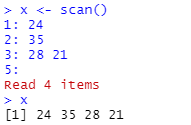
\includegraphics{Figure/scan_num.png}

문자형 벡터의 입력은 옵션 \texttt{what="character"}를 포함해야 한다.
함수 \texttt{c()}의 경우와는 다르게 각각의 자료에 인용부호를 사용할 필요는 없으나, 만일 자료에 빈칸이 포함되어 있다면 그 자료를 인용부호로 감싸야 한다.

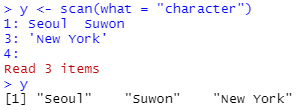
\includegraphics{Figure/scan_char.png}

한 변수의 자료가 입력되어 있는 데이터 파일을 벡터로 불러오고자 하는 경우에도 함수 \texttt{scan()}을 사용할 수 있다.
텍스트 파일에 입력된 각 자료들은 반드시 한 칸 이상의 빈 칸으로 구분되어 있어야 한다.
예를 들어 \texttt{D:\textbackslash{}Data} 폴더에 있는 파일 data1.txt에 다음과 같이 데이터가 저장되어 있다고 하자.
이것을 벡터 \texttt{z}에 입력시키는 방법은 다음과 같이 \texttt{scan()}에 불러올 파일이 저장된 위치를 입력하면 된다.

\begin{figure}
\centering
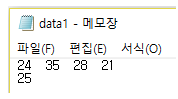
\includegraphics{Figure/data1.png}
\caption{data1.txt}
\end{figure}

\begin{Shaded}
\begin{Highlighting}[]
\SpecialCharTok{\textgreater{}}\NormalTok{ z }\OtherTok{\textless{}{-}} \FunctionTok{scan}\NormalTok{(}\StringTok{"Data/data1.txt"}\NormalTok{)}
\SpecialCharTok{\textgreater{}}\NormalTok{ z}
\NormalTok{[}\DecValTok{1}\NormalTok{] }\DecValTok{24} \DecValTok{35} \DecValTok{28} \DecValTok{21} \DecValTok{25}
\end{Highlighting}
\end{Shaded}

\hypertarget{uxb2e4uxc591uxd55c-uxd615uxd0dcuxb97c-uxac16uxb294-uxbca1uxd130uxc758-uxc0dduxc131}{%
\subsection{다양한 형태를 갖는 벡터의 생성}\label{uxb2e4uxc591uxd55c-uxd615uxd0dcuxb97c-uxac16uxb294-uxbca1uxd130uxc758-uxc0dduxc131}}

이 절에서는 기존의 벡터에 데이터를 추가하거나 여러 벡터들을 결합하여 하나의 벡터를 만드는 방법 및 일정한 구조를 갖는 벡터의 생성 방법을 살펴보겠다.

\hypertarget{uxbca1uxd130uxc5d0-uxb370uxc774uxd130-uxcd94uxac00-uxbc0f-uxbca1uxd130uxb4e4uxc758-uxacb0uxd569}{%
\subsubsection{벡터에 데이터 추가 및 벡터들의 결합}\label{uxbca1uxd130uxc5d0-uxb370uxc774uxd130-uxcd94uxac00-uxbc0f-uxbca1uxd130uxb4e4uxc758-uxacb0uxd569}}

기존의 벡터에 추가적으로 데이터를 덧붙이는 작업이나 벡터들을 결합하는 작업은 함수 \texttt{c()} 또는 함수 \texttt{append()}를 이용하여 할 수 있다. 우선 \texttt{c()}에 의한 결합 예를 살펴보자.

\begin{Shaded}
\begin{Highlighting}[]
\SpecialCharTok{\textgreater{}}\NormalTok{ x }\OtherTok{\textless{}{-}} \FunctionTok{c}\NormalTok{(}\DecValTok{11}\NormalTok{,}\DecValTok{12}\NormalTok{,}\DecValTok{13}\NormalTok{,}\DecValTok{14}\NormalTok{)}
\SpecialCharTok{\textgreater{}} \FunctionTok{c}\NormalTok{(x, }\DecValTok{15}\NormalTok{)}
\NormalTok{[}\DecValTok{1}\NormalTok{] }\DecValTok{11} \DecValTok{12} \DecValTok{13} \DecValTok{14} \DecValTok{15}
\SpecialCharTok{\textgreater{}}\NormalTok{ y }\OtherTok{\textless{}{-}} \FunctionTok{c}\NormalTok{(}\DecValTok{16}\NormalTok{,}\DecValTok{17}\NormalTok{,}\DecValTok{18}\NormalTok{)}
\SpecialCharTok{\textgreater{}} \FunctionTok{c}\NormalTok{(x, y)}
\NormalTok{[}\DecValTok{1}\NormalTok{] }\DecValTok{11} \DecValTok{12} \DecValTok{13} \DecValTok{14} \DecValTok{16} \DecValTok{17} \DecValTok{18}
\end{Highlighting}
\end{Shaded}

함수 \texttt{append()}는 추가되는 스칼라 혹은 벡터의 위치를 옵션 \texttt{after}로 지정할 수 있다.

\begin{Shaded}
\begin{Highlighting}[]
\SpecialCharTok{\textgreater{}} \FunctionTok{append}\NormalTok{(x, }\DecValTok{15}\NormalTok{)}
\NormalTok{[}\DecValTok{1}\NormalTok{] }\DecValTok{11} \DecValTok{12} \DecValTok{13} \DecValTok{14} \DecValTok{15}
\SpecialCharTok{\textgreater{}} \FunctionTok{append}\NormalTok{(x, }\DecValTok{15}\NormalTok{, }\AttributeTok{after=}\DecValTok{2}\NormalTok{)}
\NormalTok{[}\DecValTok{1}\NormalTok{] }\DecValTok{11} \DecValTok{12} \DecValTok{15} \DecValTok{13} \DecValTok{14}
\SpecialCharTok{\textgreater{}} \FunctionTok{append}\NormalTok{(x, y)}
\NormalTok{[}\DecValTok{1}\NormalTok{] }\DecValTok{11} \DecValTok{12} \DecValTok{13} \DecValTok{14} \DecValTok{16} \DecValTok{17} \DecValTok{18}
\SpecialCharTok{\textgreater{}} \FunctionTok{append}\NormalTok{(x, y, }\AttributeTok{after=}\DecValTok{3}\NormalTok{)}
\NormalTok{[}\DecValTok{1}\NormalTok{] }\DecValTok{11} \DecValTok{12} \DecValTok{13} \DecValTok{16} \DecValTok{17} \DecValTok{18} \DecValTok{14}
\end{Highlighting}
\end{Shaded}

\hypertarget{uxc77cuxc815uxd55c-uxad6cuxc870uxb97c-uxac16uxb294-uxbca1uxd130uxc758-uxc0dduxc131}{%
\subsubsection{일정한 구조를 갖는 벡터의 생성}\label{uxc77cuxc815uxd55c-uxad6cuxc870uxb97c-uxac16uxb294-uxbca1uxd130uxc758-uxc0dduxc131}}

일정한 구조를 갖고 있는 벡터가 필요한 경우가 있다. 예를 들어 1부터 100까지의 정수로 이루어진 벡터를 만들어야 한다고 하자. 이러한 경우 \texttt{c()}에 숫자를 하나하나 입력해야 한다면 무척 한심스러운 일이 될 것이다.
\texttt{콜론(:)} 연산자 또는 \texttt{seq()}를 이용하면 일정한 간격이 있는 자료를 쉽게 만들 수 있으며, \texttt{rep()}를 이용하면 반복된 패턴이 있는 자료를 간편하게 만들 수 있다.

\begin{itemize}
\tightlist
\item
  콜론 연산자
\end{itemize}

콜론 연산자는 연산자의 왼쪽 숫자에서 시작하여 오른쪽 숫자를 초과하지 않을 때까지 1씩 증가하는 수열을 만든다. 왼쪽의 숫자가 오른쪽의 숫자보다 크면 1씩 감소를 시킨다.

\begin{Shaded}
\begin{Highlighting}[]
\SpecialCharTok{\textgreater{}} \DecValTok{1}\SpecialCharTok{:}\DecValTok{5}
\NormalTok{[}\DecValTok{1}\NormalTok{] }\DecValTok{1} \DecValTok{2} \DecValTok{3} \DecValTok{4} \DecValTok{5}
\SpecialCharTok{\textgreater{}} \SpecialCharTok{{-}}\DecValTok{3}\SpecialCharTok{:}\DecValTok{3}
\NormalTok{[}\DecValTok{1}\NormalTok{] }\SpecialCharTok{{-}}\DecValTok{3} \SpecialCharTok{{-}}\DecValTok{2} \SpecialCharTok{{-}}\DecValTok{1}  \DecValTok{0}  \DecValTok{1}  \DecValTok{2}  \DecValTok{3}
\SpecialCharTok{\textgreater{}} \FloatTok{1.5}\SpecialCharTok{:}\FloatTok{5.4}
\NormalTok{[}\DecValTok{1}\NormalTok{] }\FloatTok{1.5} \FloatTok{2.5} \FloatTok{3.5} \FloatTok{4.5}
\SpecialCharTok{\textgreater{}} \DecValTok{5}\SpecialCharTok{:}\DecValTok{0}
\NormalTok{[}\DecValTok{1}\NormalTok{] }\DecValTok{5} \DecValTok{4} \DecValTok{3} \DecValTok{2} \DecValTok{1} \DecValTok{0}
\end{Highlighting}
\end{Shaded}

\begin{itemize}
\tightlist
\item
  함수 \texttt{seq()}에 의한 수열 생성
\end{itemize}

콜론 연산자는 만들고자 하는 수열의 증가 폭이 1인 경우에만 사용할 수 있다는 한계가 있다. 조금 더 일반적인 형태의 수열을 만드는 작업은 함수 \texttt{seq()}를 사용해야 한다.
가장 기본적인 형태는 옵션 \texttt{from}과 \texttt{to}가 있으면서 \texttt{by}와 \texttt{length}로 수열의 간격 또는 개수를 지정하는 것이다. 시작점(from)과 끝점(to)만이 있다면, 콜론 연산자의 경우와 같이 간격이 1이 된다. 옵션 \texttt{by}는 간격을 지정하는 것으로써 \texttt{from}에서 시작하여 \texttt{by} 만큼 증가(감소)를 시키되 \texttt{to}를 지나치지 않는 수열을 생성한다. 옵션 \texttt{length}는 수열의 개수를 지정하는 것으로써 \texttt{from}과 \texttt{to}를 포함하는 간격이 일정한 수열을 생성한다. 만일 옵션 \texttt{to}가 없다면, \texttt{from}에서 시작하여 \texttt{by} 만큼의 간격이 있는 \texttt{length}개의 수열을 구성한다.

\begin{Shaded}
\begin{Highlighting}[]
\SpecialCharTok{\textgreater{}} \FunctionTok{seq}\NormalTok{(}\AttributeTok{from=}\DecValTok{0}\NormalTok{, }\AttributeTok{to=}\DecValTok{5}\NormalTok{)   }
\NormalTok{[}\DecValTok{1}\NormalTok{] }\DecValTok{0} \DecValTok{1} \DecValTok{2} \DecValTok{3} \DecValTok{4} \DecValTok{5}
\SpecialCharTok{\textgreater{}} \FunctionTok{seq}\NormalTok{(}\AttributeTok{from=}\DecValTok{0}\NormalTok{, }\AttributeTok{to=}\DecValTok{5}\NormalTok{, }\AttributeTok{by=}\DecValTok{2}\NormalTok{)}
\NormalTok{[}\DecValTok{1}\NormalTok{] }\DecValTok{0} \DecValTok{2} \DecValTok{4}
\SpecialCharTok{\textgreater{}} \FunctionTok{seq}\NormalTok{(}\AttributeTok{from=}\DecValTok{0}\NormalTok{, }\AttributeTok{to=}\DecValTok{5}\NormalTok{, }\AttributeTok{length=}\DecValTok{3}\NormalTok{)}
\NormalTok{[}\DecValTok{1}\NormalTok{] }\FloatTok{0.0} \FloatTok{2.5} \FloatTok{5.0}
\SpecialCharTok{\textgreater{}} \FunctionTok{seq}\NormalTok{(}\AttributeTok{from=}\DecValTok{0}\NormalTok{, }\AttributeTok{by=}\DecValTok{2}\NormalTok{, }\AttributeTok{length=}\DecValTok{3}\NormalTok{)}
\NormalTok{[}\DecValTok{1}\NormalTok{] }\DecValTok{0} \DecValTok{2} \DecValTok{4}
\end{Highlighting}
\end{Shaded}

함수 \texttt{seq()}에 하나의 숫자만을 입력하면 1을 시작점으로 하여 1씩 증가(감소)하여 지정된 숫자를 끝점으로 하는 수열이 만들어진다.

\begin{Shaded}
\begin{Highlighting}[]
\SpecialCharTok{\textgreater{}} \FunctionTok{seq}\NormalTok{(}\DecValTok{3}\NormalTok{)}
\NormalTok{[}\DecValTok{1}\NormalTok{] }\DecValTok{1} \DecValTok{2} \DecValTok{3}
\SpecialCharTok{\textgreater{}} \FunctionTok{seq}\NormalTok{(}\SpecialCharTok{{-}}\DecValTok{3}\NormalTok{)}
\NormalTok{[}\DecValTok{1}\NormalTok{]  }\DecValTok{1}  \DecValTok{0} \SpecialCharTok{{-}}\DecValTok{1} \SpecialCharTok{{-}}\DecValTok{2} \SpecialCharTok{{-}}\DecValTok{3}
\end{Highlighting}
\end{Shaded}

주어진 벡터와 길이가 같으면서, 1에서부터 시작하고 간격이 1인 수열이 필요한 경우가 있다. 이러한 경우에는 함수 \texttt{seq()}의 옵션 \texttt{along}에 해당되는 벡터를 지정하거나, 옵션 \texttt{length}에 해당 벡터의 길이를 지정하면 된다. 또는 함수 \texttt{seq\_along()} 혹은 함수 \texttt{seq\_len()}을 대신 사용해도 된다.

\begin{Shaded}
\begin{Highlighting}[]
\SpecialCharTok{\textgreater{}}\NormalTok{ x }\OtherTok{\textless{}{-}} \FunctionTok{c}\NormalTok{(}\DecValTok{24}\NormalTok{,}\DecValTok{31}\NormalTok{,}\DecValTok{29}\NormalTok{)}
\SpecialCharTok{\textgreater{}} \FunctionTok{seq}\NormalTok{(}\AttributeTok{along=}\NormalTok{x)}
\NormalTok{[}\DecValTok{1}\NormalTok{] }\DecValTok{1} \DecValTok{2} \DecValTok{3}
\SpecialCharTok{\textgreater{}} \FunctionTok{seq\_along}\NormalTok{(x)}
\NormalTok{[}\DecValTok{1}\NormalTok{] }\DecValTok{1} \DecValTok{2} \DecValTok{3}
\SpecialCharTok{\textgreater{}} \FunctionTok{seq}\NormalTok{(}\AttributeTok{length=}\FunctionTok{length}\NormalTok{(x))}
\NormalTok{[}\DecValTok{1}\NormalTok{] }\DecValTok{1} \DecValTok{2} \DecValTok{3}
\SpecialCharTok{\textgreater{}} \FunctionTok{seq\_len}\NormalTok{(}\FunctionTok{length}\NormalTok{(x))}
\NormalTok{[}\DecValTok{1}\NormalTok{] }\DecValTok{1} \DecValTok{2} \DecValTok{3}
\end{Highlighting}
\end{Shaded}

\begin{itemize}
\tightlist
\item
  함수 \texttt{rep()}에 의한 반복된 패턴이 있는 데이터 생성
\end{itemize}

함수 \texttt{rep()}는 옵션 \texttt{times}와 \texttt{each}, \texttt{length}를 이용하여 다양한 형태의 반복된 패턴이 있는 데이터를 만들 수 있다. 옵션 \texttt{times}는 반복 횟수를 지정하는 것으로써 하나의 정수를 지정할 때와 반복시키려는 벡터의 길이와 같은 정수형 벡터를 지정할 때에 다른 결과가 나온다.

\begin{Shaded}
\begin{Highlighting}[]
\SpecialCharTok{\textgreater{}} \FunctionTok{rep}\NormalTok{(}\DecValTok{1}\NormalTok{, }\AttributeTok{times=}\DecValTok{3}\NormalTok{)     }
\NormalTok{[}\DecValTok{1}\NormalTok{] }\DecValTok{1} \DecValTok{1} \DecValTok{1}
\SpecialCharTok{\textgreater{}} \FunctionTok{rep}\NormalTok{(}\DecValTok{1}\SpecialCharTok{:}\DecValTok{3}\NormalTok{, }\AttributeTok{times=}\DecValTok{2}\NormalTok{)}
\NormalTok{[}\DecValTok{1}\NormalTok{] }\DecValTok{1} \DecValTok{2} \DecValTok{3} \DecValTok{1} \DecValTok{2} \DecValTok{3}
\SpecialCharTok{\textgreater{}} \FunctionTok{rep}\NormalTok{(}\FunctionTok{c}\NormalTok{(}\StringTok{"M"}\NormalTok{,}\StringTok{"F"}\NormalTok{), }\AttributeTok{times=}\FunctionTok{c}\NormalTok{(}\DecValTok{2}\NormalTok{,}\DecValTok{3}\NormalTok{))}
\NormalTok{[}\DecValTok{1}\NormalTok{] }\StringTok{"M"} \StringTok{"M"} \StringTok{"F"} \StringTok{"F"} \StringTok{"F"}
\end{Highlighting}
\end{Shaded}

옵션 \texttt{times}에 하나의 반복 횟수만 지정하면 데이터 전체를 지정된 횟수만큼 반복시킨다. 반복 대상이 \texttt{c("M","F")}이고 반복 횟수가 \texttt{c(2,3)}이 되어 일대일 대응이 되는 경우에는 \texttt{M}이 두 번 먼저 반복되고 이어서 \texttt{F}가 세 번 반복된다.

옵션 \texttt{each}에 반복 횟수를 지정하면, 데이터의 요소들이 각각 each번 반복한다. 이어서 옵션 \texttt{times}를 추가하면 각 요소의 \texttt{each}번 반복 과정 전체가 \texttt{times}만큼 반복된다.

\begin{Shaded}
\begin{Highlighting}[]
\SpecialCharTok{\textgreater{}} \FunctionTok{rep}\NormalTok{(}\DecValTok{1}\SpecialCharTok{:}\DecValTok{3}\NormalTok{, }\AttributeTok{each=}\DecValTok{2}\NormalTok{)}
\NormalTok{[}\DecValTok{1}\NormalTok{] }\DecValTok{1} \DecValTok{1} \DecValTok{2} \DecValTok{2} \DecValTok{3} \DecValTok{3}
\SpecialCharTok{\textgreater{}} \FunctionTok{rep}\NormalTok{(}\DecValTok{1}\SpecialCharTok{:}\DecValTok{3}\NormalTok{, }\AttributeTok{times=}\FunctionTok{rep}\NormalTok{(}\DecValTok{2}\NormalTok{,}\DecValTok{3}\NormalTok{))}
\NormalTok{[}\DecValTok{1}\NormalTok{] }\DecValTok{1} \DecValTok{1} \DecValTok{2} \DecValTok{2} \DecValTok{3} \DecValTok{3}
\SpecialCharTok{\textgreater{}} \FunctionTok{rep}\NormalTok{(}\DecValTok{1}\SpecialCharTok{:}\DecValTok{3}\NormalTok{, }\AttributeTok{each=}\DecValTok{2}\NormalTok{, }\AttributeTok{times=}\DecValTok{2}\NormalTok{)}
\NormalTok{ [}\DecValTok{1}\NormalTok{] }\DecValTok{1} \DecValTok{1} \DecValTok{2} \DecValTok{2} \DecValTok{3} \DecValTok{3} \DecValTok{1} \DecValTok{1} \DecValTok{2} \DecValTok{2} \DecValTok{3} \DecValTok{3}
\end{Highlighting}
\end{Shaded}

옵션 \texttt{length}에 벡터의 길이를 지정하면, 길이가 \texttt{length}가 될 때까지 데이터 전체가 반복된다. 옵션 \texttt{each}를 함께 사용하면, 데이터 각 요소가 \texttt{each}번 반복되는 과정을 반복하여 결과 벡터의 길이가 \texttt{length}가 되도록 한다.

\begin{Shaded}
\begin{Highlighting}[]
\SpecialCharTok{\textgreater{}} \FunctionTok{rep}\NormalTok{(}\DecValTok{1}\SpecialCharTok{:}\DecValTok{3}\NormalTok{, }\AttributeTok{length=}\DecValTok{6}\NormalTok{)}
\NormalTok{[}\DecValTok{1}\NormalTok{] }\DecValTok{1} \DecValTok{2} \DecValTok{3} \DecValTok{1} \DecValTok{2} \DecValTok{3}
\SpecialCharTok{\textgreater{}} \FunctionTok{rep}\NormalTok{(}\DecValTok{1}\SpecialCharTok{:}\DecValTok{3}\NormalTok{, }\AttributeTok{each=}\DecValTok{2}\NormalTok{, }\AttributeTok{length=}\DecValTok{8}\NormalTok{)}
\NormalTok{[}\DecValTok{1}\NormalTok{] }\DecValTok{1} \DecValTok{1} \DecValTok{2} \DecValTok{2} \DecValTok{3} \DecValTok{3} \DecValTok{1} \DecValTok{1}
\end{Highlighting}
\end{Shaded}

\hypertarget{uxbb38uxc790uxc5f4uxc744-uxc704uxd55c-uxd568uxc218}{%
\subsection{문자열을 위한 함수}\label{uxbb38uxc790uxc5f4uxc744-uxc704uxd55c-uxd568uxc218}}

R에는 문자열을 다루기 위한 매우 유용한 함수들이 있다. 우리는 종종 문자형 벡터에서 특
정 정보를 얻거나 문자형 벡터의 내용을 수정해야 할 때가 있는데 이런 경우 유용하게 사
용할 수 있는 함수들이 Table \ref{tab:char-func}에 있다.

\begin{longtable}[]{@{}ll@{}}
\caption{\label{tab:char-func}문자 함수}\tabularnewline
\toprule
함수 & 기능 \\
\midrule
\endfirsthead
\toprule
함수 & 기능 \\
\midrule
\endhead
nchar(x) & 문자열 x를 구성하는 문자의 개수 \\
paste(\ldots, sep='' ``) & 문자열의 결합 \\
substr(x, start, stop) & 문자열 일부분 선택 \\
toupper(x) & 영문자 대문자로 변환 \\
tolower(x) & 영문자 소문자로 변환 \\
strsplit(x, split) & 문자열의 분리 \\
sub(old, new, x) & 문자열 치환 \\
gsub(old, new, x) & 문자열 치환 \\
\bottomrule
\end{longtable}

\begin{itemize}
\tightlist
\item
  함수 \texttt{nchar()}: 문자열을 구성하는 문자 개수 계산
\end{itemize}

함수 \texttt{nchar()}는 문자열을 구성하고 있는 문자의 개수를 센다. 다음에 주어진 문자형 벡터
\texttt{x}의 첫 문자열은 4개, 두 번째는 3개, 마지막 문자열은 4개의 문자로 이루어졌다는 것을
알 수 있다. 한글로 이루어진 문자열도 문제 없이 문자 개수를 셀 수 있다.

\begin{Shaded}
\begin{Highlighting}[]
\SpecialCharTok{\textgreater{}}\NormalTok{ x }\OtherTok{\textless{}{-}} \FunctionTok{c}\NormalTok{(}\StringTok{"Park"}\NormalTok{,}\StringTok{"Lee"}\NormalTok{,}\StringTok{"Kwon"}\NormalTok{)}
\SpecialCharTok{\textgreater{}} \FunctionTok{nchar}\NormalTok{(x)}
\NormalTok{[}\DecValTok{1}\NormalTok{] }\DecValTok{4} \DecValTok{3} \DecValTok{4}
\SpecialCharTok{\textgreater{}} \FunctionTok{nchar}\NormalTok{(}\StringTok{"응용통계학과"}\NormalTok{)}
\NormalTok{[}\DecValTok{1}\NormalTok{] }\DecValTok{6}
\end{Highlighting}
\end{Shaded}

\begin{itemize}
\tightlist
\item
  함수 \texttt{paste()}: 문자열의 결합
\end{itemize}

여러 개의 문자열들을 적절하게 결합시켜 새로운 문자열을 만들어야 하는 경우가 자주 있
다. 이런 경우에 함수 \texttt{paste()}가 매우 유용하게 사용된다. 함수 \texttt{paste()}의 기본적인 사용법은 결합시키고자 하는 문자열들을 차례로 입력하는 것이고, 옵션 \texttt{sep}에서 지정하는 문자 혹은 빈칸 등이 결합되는 문자열과 문자열 사이에 오게 된다.

5개의 문자열인 ``모든'', ``사람에게는'', ``통계적'', ``사고능력이'' 그리고 ``필요하다''를 결
합시켜 보자. 첫 번째는 옵션 \texttt{sep}의 디폴트 값인 \texttt{sep="\ "}가 사용되어 결합되는 문자열들
사이에 하나의 빈칸이 생긴 것이고, 두 번째는 \texttt{sep="-"}가 지정되어 문자열들이 대시(dash)
기호로 결합되었고, 세 번째에는 \texttt{sep=""}이 사용되어 빈칸 없이 문자열들이 결합되었다.

\begin{Shaded}
\begin{Highlighting}[]
\SpecialCharTok{\textgreater{}} \FunctionTok{paste}\NormalTok{(}\StringTok{"모든"}\NormalTok{, }\StringTok{"사람에게는"}\NormalTok{, }\StringTok{"통계적"}\NormalTok{, }\StringTok{"사고능력이"}\NormalTok{, }\StringTok{"필요하다"}\NormalTok{)}
\NormalTok{[}\DecValTok{1}\NormalTok{] }\StringTok{"모든 사람에게는 통계적 사고능력이 필요하다"}
\SpecialCharTok{\textgreater{}} \FunctionTok{paste}\NormalTok{(}\StringTok{"모든"}\NormalTok{, }\StringTok{"사람에게는"}\NormalTok{, }\StringTok{"통계적"}\NormalTok{, }\StringTok{"사고능력이"}\NormalTok{, }\StringTok{"필요하다"}\NormalTok{,}
\SpecialCharTok{+}       \AttributeTok{sep=}\StringTok{"{-}"}\NormalTok{)}
\NormalTok{[}\DecValTok{1}\NormalTok{] }\StringTok{"모든{-}사람에게는{-}통계적{-}사고능력이{-}필요하다"}
\SpecialCharTok{\textgreater{}} \FunctionTok{paste}\NormalTok{(}\StringTok{"모든"}\NormalTok{, }\StringTok{"사람에게는"}\NormalTok{, }\StringTok{"통계적"}\NormalTok{, }\StringTok{"사고능력이"}\NormalTok{, }\StringTok{"필요하다"}\NormalTok{,}
\SpecialCharTok{+}       \AttributeTok{sep=}\StringTok{""}\NormalTok{)}
\NormalTok{[}\DecValTok{1}\NormalTok{] }\StringTok{"모든사람에게는통계적사고능력이필요하다"}
\end{Highlighting}
\end{Shaded}

함수 \texttt{paste()}에 입력된 숫자는 문자로 전환되어 문자열 결합에 사용된다.

\begin{Shaded}
\begin{Highlighting}[]
\SpecialCharTok{\textgreater{}} \FunctionTok{paste}\NormalTok{(}\StringTok{"원주율은"}\NormalTok{, pi, }\StringTok{"이다"}\NormalTok{)}
\NormalTok{[}\DecValTok{1}\NormalTok{] }\StringTok{"원주율은 3.14159265358979 이다"}
\end{Highlighting}
\end{Shaded}

함수 \texttt{paste()} 안에 문자형 벡터 몇 개가 함께 들어오면 벡터들의 대응되는 요소끼리의
결합이 이루어진다. 이때 벡터의 길이가 서로 다르면, 순환법칙이 적용된다. 즉, 문자열
\texttt{"Stat"}과 벡터 \texttt{1:3}을 함께 입력하면 실제로는 \texttt{c("Stat","Stat","Stat")}과 \texttt{1:3}이 결합이 되는 것이고, \texttt{c("Stat","Math")}와 \texttt{1:3}을 함께 입력하면, \texttt{c("Stat","Math",\ "Stat")}과 \texttt{1:3}이 결합되는 것이다.

\begin{Shaded}
\begin{Highlighting}[]
\SpecialCharTok{\textgreater{}} \FunctionTok{paste}\NormalTok{(}\FunctionTok{c}\NormalTok{(}\StringTok{"Stat"}\NormalTok{, }\StringTok{"Math"}\NormalTok{), }\DecValTok{1}\SpecialCharTok{:}\DecValTok{2}\NormalTok{, }\AttributeTok{sep =} \StringTok{""}\NormalTok{)}
\NormalTok{[}\DecValTok{1}\NormalTok{] }\StringTok{"Stat1"} \StringTok{"Math2"}
\SpecialCharTok{\textgreater{}} \FunctionTok{paste}\NormalTok{(}\StringTok{"Stat"}\NormalTok{, }\DecValTok{1}\SpecialCharTok{:}\DecValTok{3}\NormalTok{, }\AttributeTok{sep=}\StringTok{""}\NormalTok{)}
\NormalTok{[}\DecValTok{1}\NormalTok{] }\StringTok{"Stat1"} \StringTok{"Stat2"} \StringTok{"Stat3"}
\SpecialCharTok{\textgreater{}} \FunctionTok{paste}\NormalTok{(}\FunctionTok{c}\NormalTok{(}\StringTok{"Stat"}\NormalTok{,}\StringTok{"Math"}\NormalTok{), }\DecValTok{1}\SpecialCharTok{:}\DecValTok{3}\NormalTok{, }\AttributeTok{sep=}\StringTok{"{-}"}\NormalTok{)}
\NormalTok{[}\DecValTok{1}\NormalTok{] }\StringTok{"Stat{-}1"} \StringTok{"Math{-}2"} \StringTok{"Stat{-}3"}
\end{Highlighting}
\end{Shaded}

빈칸 없이 문자열을 결합시킬 때에는 함수 \texttt{paste()}에 옵션 \texttt{sep=""}을 추가하는 것보다
그냥 함수 \texttt{paste0()}을 사용하는 것이 더 편리하다.

\begin{Shaded}
\begin{Highlighting}[]
\SpecialCharTok{\textgreater{}} \FunctionTok{paste0}\NormalTok{(}\StringTok{"stat"}\NormalTok{, }\DecValTok{1}\SpecialCharTok{:}\DecValTok{3}\NormalTok{)}
\NormalTok{[}\DecValTok{1}\NormalTok{] }\StringTok{"stat1"} \StringTok{"stat2"} \StringTok{"stat3"}
\end{Highlighting}
\end{Shaded}

한 개의 문자형 벡터를 구성하고 있는 모든 문자열을 묶어서 하나의 문자열로 나타내는
작업이 필요한 경우가 있다. 이때는 옵션 \texttt{collapse}를 사용하면 된다. 영문자 소문자와 대문자로 구성된 문자형 벡터 \texttt{letters}와 \texttt{LETTERS}를 각각 하나의 문자열로 합쳐보자.

\begin{Shaded}
\begin{Highlighting}[]
\SpecialCharTok{\textgreater{}}\NormalTok{ letters}
\NormalTok{ [}\DecValTok{1}\NormalTok{] }\StringTok{"a"} \StringTok{"b"} \StringTok{"c"} \StringTok{"d"} \StringTok{"e"} \StringTok{"f"} \StringTok{"g"} \StringTok{"h"} \StringTok{"i"} \StringTok{"j"} \StringTok{"k"} \StringTok{"l"} \StringTok{"m"} \StringTok{"n"} \StringTok{"o"} \StringTok{"p"} \StringTok{"q"} \StringTok{"r"} \StringTok{"s"}
\NormalTok{[}\DecValTok{20}\NormalTok{] }\StringTok{"t"} \StringTok{"u"} \StringTok{"v"} \StringTok{"w"} \StringTok{"x"} \StringTok{"y"} \StringTok{"z"}
\SpecialCharTok{\textgreater{}} \FunctionTok{paste0}\NormalTok{(letters, }\AttributeTok{collapse=}\StringTok{""}\NormalTok{)}
\NormalTok{[}\DecValTok{1}\NormalTok{] }\StringTok{"abcdefghijklmnopqrstuvwxyz"}
\SpecialCharTok{\textgreater{}} \FunctionTok{paste}\NormalTok{(LETTERS, }\AttributeTok{collapse=}\StringTok{","}\NormalTok{)}
\NormalTok{[}\DecValTok{1}\NormalTok{] }\StringTok{"A,B,C,D,E,F,G,H,I,J,K,L,M,N,O,P,Q,R,S,T,U,V,W,X,Y,Z"}
\end{Highlighting}
\end{Shaded}

하나의 문자열로 합쳐질 때 옵션 \texttt{collapse}에 지정한 문자가 일종의 구분자 역할을 하고
있다.

함수 \texttt{paste()}에 두 개의 문자형 벡터를 입력하고, 이어서 옵션 \texttt{collapse}를 사용하면 입력된 두 문자형 벡터를 하나의 문자형 벡터로 결합시키고, 이어서 모든 문자열을 묶어서 하나의 문자열로 나타낸다.

\begin{Shaded}
\begin{Highlighting}[]
\SpecialCharTok{\textgreater{}} \FunctionTok{paste0}\NormalTok{(letters, LETTERS, }\AttributeTok{collapse =} \StringTok{","}\NormalTok{)}
\NormalTok{[}\DecValTok{1}\NormalTok{] }\StringTok{"aA,bB,cC,dD,eE,fF,gG,hH,iI,jJ,kK,lL,mM,nN,oO,pP,qQ,rR,sS,tT,uU,vV,wW,xX,yY,zZ"}
\SpecialCharTok{\textgreater{}} \FunctionTok{paste}\NormalTok{(letters, LETTERS, }\AttributeTok{sep =} \StringTok{"{-}"}\NormalTok{, }\AttributeTok{collapse =} \StringTok{","}\NormalTok{)}
\NormalTok{[}\DecValTok{1}\NormalTok{] }\StringTok{"a{-}A,b{-}B,c{-}C,d{-}D,e{-}E,f{-}F,g{-}G,h{-}H,i{-}I,j{-}J,k{-}K,l{-}L,m{-}M,n{-}N,o{-}O,p{-}P,q{-}Q,r{-}R,s{-}S,t{-}T,u{-}U,v{-}V,w{-}W,x{-}X,y{-}Y,z{-}Z"}
\end{Highlighting}
\end{Shaded}

\begin{itemize}
\tightlist
\item
  함수 \texttt{substr()}: 문자열에서 일부분 선택
\end{itemize}

주어진 문자열에서 일부분을 선택해야 하는 작업도 빈번히 일어나는 중요한 작업 중 하나
이다. 함수 \texttt{substr()}에는 문자형 벡터, 시작점, 끝점이 차례로 입력된다. 시작점과 끝점은
각각 정수형 스칼라 혹은 벡터가 된다.

시작점과 끝점이 벡터가 되면, 대응되는 숫자끼리 시작점과 끝점을 구성하며 필요하다면 순환법칙도 적용된다.
아래 예의 첫 번째 결과는 문자형 벡터 \texttt{x}를 구성하고 있는 세 문자에 대하여 동일하게
시작점과 끝점을 하나의 숫자로 지정하여 추출한 것이다. 두 번째 결과는 시작점과 끝점이
벡터로 지정된 것으로 첫 번째 문자열에는 (시작점=1, 끝점=2), 두 번째 문자열에는 (시작
점=3, 끝점=6), 그리고 세 번째 문자열에는 다시 (시작점=1, 끝점=2)가 적용된 결과이다.

\begin{Shaded}
\begin{Highlighting}[]
\SpecialCharTok{\textgreater{}} \FunctionTok{substr}\NormalTok{(}\StringTok{"Statistics"}\NormalTok{, }\DecValTok{1}\NormalTok{, }\DecValTok{4}\NormalTok{)}
\NormalTok{[}\DecValTok{1}\NormalTok{] }\StringTok{"Stat"}
\SpecialCharTok{\textgreater{}}\NormalTok{ x }\OtherTok{\textless{}{-}} \FunctionTok{c}\NormalTok{(}\StringTok{"응용통계학과"}\NormalTok{, }\StringTok{"정보통계학과"}\NormalTok{, }\StringTok{"학생회장"}\NormalTok{) }
\SpecialCharTok{\textgreater{}} \FunctionTok{substr}\NormalTok{(x, }\DecValTok{3}\NormalTok{, }\DecValTok{6}\NormalTok{)}
\NormalTok{[}\DecValTok{1}\NormalTok{] }\StringTok{"통계학과"} \StringTok{"통계학과"} \StringTok{"회장"}    
\SpecialCharTok{\textgreater{}} \FunctionTok{substr}\NormalTok{(x, }\FunctionTok{c}\NormalTok{(}\DecValTok{1}\NormalTok{,}\DecValTok{3}\NormalTok{), }\FunctionTok{c}\NormalTok{(}\DecValTok{2}\NormalTok{,}\DecValTok{6}\NormalTok{))}
\NormalTok{[}\DecValTok{1}\NormalTok{] }\StringTok{"응용"}     \StringTok{"통계학과"} \StringTok{"학생"}    
\end{Highlighting}
\end{Shaded}

미국의 세 도시와 그 도시가 속한 주 이름이 입력된 문자형 벡터 \texttt{x}에서 세 도시가 속한
주 이름만을 선택하여 출력해 보자. 비록 세 문자열의 길이가 서로 다르지만 주의 이름은
각 문자열의 마지막 두 칸에 있다는 점에 착안하여 함수 \texttt{nchar()}로 시작점과 끝점을 지정할 수 있다.

\begin{Shaded}
\begin{Highlighting}[]
\SpecialCharTok{\textgreater{}}\NormalTok{ x }\OtherTok{\textless{}{-}} \FunctionTok{c}\NormalTok{(}\StringTok{"New York, NY"}\NormalTok{,}\StringTok{"Ann Arbor, MI"}\NormalTok{,}\StringTok{"Chicago, IL"}\NormalTok{)}
\SpecialCharTok{\textgreater{}} \FunctionTok{substr}\NormalTok{(x, }\AttributeTok{start=}\FunctionTok{nchar}\NormalTok{(x)}\SpecialCharTok{{-}}\DecValTok{1}\NormalTok{, }\AttributeTok{stop=}\FunctionTok{nchar}\NormalTok{(x))}
\NormalTok{[}\DecValTok{1}\NormalTok{] }\StringTok{"NY"} \StringTok{"MI"} \StringTok{"IL"}
\end{Highlighting}
\end{Shaded}

패키지 \texttt{ggplot2}에 있는 데이터 프레임 \texttt{mpg}는 자동차의 연비와 관련된 자료이다. 11개의
변수 중 \texttt{trans}는 변속기 종류를 나타내는 변수이다. 변수 \texttt{trans}가 갖는 값을 살펴보자. 함수 \texttt{library()}로 패키지를 로딩하지 않은 상태에서 해당 패키지의 데이터를 불러오려면
\texttt{패키지::데이터}의 형식을 사용하면 된다. \texttt{mpg\$trans}는 데이터 프레임 \texttt{mpg}의 변수 \texttt{trans}를 벡터 형태로 선택한 것이며 자세한 설명은 \ref{section-dataframe}절에서 찾아볼 수 있다.
또한 함수 \texttt{table()}로 문자형 벡터를 구성하고 있는 각 문자열의 빈도를 계산할 수 있다.

\begin{Shaded}
\begin{Highlighting}[]
\SpecialCharTok{\textgreater{}}\NormalTok{ x }\OtherTok{\textless{}{-}}\NormalTok{ ggplot2}\SpecialCharTok{::}\NormalTok{mpg}\SpecialCharTok{$}\NormalTok{trans}
\SpecialCharTok{\textgreater{}} \FunctionTok{table}\NormalTok{(x)}
\NormalTok{x}
  \FunctionTok{auto}\NormalTok{(av)   }\FunctionTok{auto}\NormalTok{(l3)   }\FunctionTok{auto}\NormalTok{(l4)   }\FunctionTok{auto}\NormalTok{(l5)   }\FunctionTok{auto}\NormalTok{(l6)   }\FunctionTok{auto}\NormalTok{(s4)   }\FunctionTok{auto}\NormalTok{(s5) }
         \DecValTok{5}          \DecValTok{2}         \DecValTok{83}         \DecValTok{39}          \DecValTok{6}          \DecValTok{3}          \DecValTok{3} 
  \FunctionTok{auto}\NormalTok{(s6) }\FunctionTok{manual}\NormalTok{(m5) }\FunctionTok{manual}\NormalTok{(m6) }
        \DecValTok{16}         \DecValTok{58}         \DecValTok{19} 
\end{Highlighting}
\end{Shaded}

auto(av)부터 auto(s6)까지를 auto로 통합하고 manual(m5)와 manual(m6)를 manual
로 통합하는 작업은 시작점을 \texttt{1}, 끝점을 \texttt{nchar(x)-4}로 지정함으로써 가능하다.

\begin{Shaded}
\begin{Highlighting}[]
\SpecialCharTok{\textgreater{}}\NormalTok{ y }\OtherTok{\textless{}{-}} \FunctionTok{substr}\NormalTok{(x, }\AttributeTok{start=}\DecValTok{1}\NormalTok{, }\AttributeTok{stop=}\FunctionTok{nchar}\NormalTok{(x)}\SpecialCharTok{{-}}\DecValTok{4}\NormalTok{)}
\SpecialCharTok{\textgreater{}} \FunctionTok{table}\NormalTok{(y)}
\NormalTok{y}
\NormalTok{  auto manual }
   \DecValTok{157}     \DecValTok{77} 
\end{Highlighting}
\end{Shaded}

\begin{itemize}
\tightlist
\item
  함수 \texttt{strsplit()}: 문자열의 분할
\end{itemize}

여러 문자열들을 서로 결합하는 것도 중요한 작업이지만 하나의 문자열을 몇 개로 분리하
는 것도 매우 중요한 작업이다. 함수 \texttt{strsplit()}는 주어진 문자열을 옵션 \texttt{split}에 지정된 기준에 의하여 분리시킨다.

문자형 벡터 \texttt{x}에 입력된 세 도시의 이름과 주 이름을 분리해 보자. 도시 이름과 주 이름
이 콤마로 구분되어 있기 때문에 분리기준으로 옵션 \texttt{split=","}을 지정하였다. 결과는 리스트로 출력된다. R 데이터 구조 중 하나인 리스트에 대한 소개는 \ref{section-list}절에 있다.

\begin{Shaded}
\begin{Highlighting}[]
\SpecialCharTok{\textgreater{}}\NormalTok{ x }\OtherTok{\textless{}{-}} \FunctionTok{c}\NormalTok{(}\StringTok{"New York, NY"}\NormalTok{,}\StringTok{"Ann Arbor, MI"}\NormalTok{,}\StringTok{"Chicago, IL"}\NormalTok{)}
\SpecialCharTok{\textgreater{}}\NormalTok{ (y }\OtherTok{\textless{}{-}} \FunctionTok{strsplit}\NormalTok{(x,}\AttributeTok{split=}\StringTok{","}\NormalTok{))}
\NormalTok{[[}\DecValTok{1}\NormalTok{]]}
\NormalTok{[}\DecValTok{1}\NormalTok{] }\StringTok{"New York"} \StringTok{" NY"}     

\NormalTok{[[}\DecValTok{2}\NormalTok{]]}
\NormalTok{[}\DecValTok{1}\NormalTok{] }\StringTok{"Ann Arbor"} \StringTok{" MI"}      

\NormalTok{[[}\DecValTok{3}\NormalTok{]]}
\NormalTok{[}\DecValTok{1}\NormalTok{] }\StringTok{"Chicago"} \StringTok{" IL"}    
\SpecialCharTok{\textgreater{}} \FunctionTok{unlist}\NormalTok{(y)}
\NormalTok{[}\DecValTok{1}\NormalTok{] }\StringTok{"New York"}  \StringTok{" NY"}       \StringTok{"Ann Arbor"} \StringTok{" MI"}       \StringTok{"Chicago"}   \StringTok{" IL"}      
\end{Highlighting}
\end{Shaded}

리스트 \texttt{y}를 생성하는 할당문 전체가 괄호로 감싸여 있는데, 이렇게 할당문을 괄호로 감싸면 할당된 객체의 값이 출력됨을 볼 수 있다. 또한 리스트 객체를 함수 \texttt{unlist()}에 입력하면, 리스트의 모든 구성요소들로 이루어진 벡터가 만들어진다.

문자열을 구성하는 개별 문자들을 모두 분리시키는 작업도 가능한데, 이 경우에는 분리
기준이 옵션 \texttt{split\ =\ ""}이 되어야 한다.

\begin{Shaded}
\begin{Highlighting}[]
\SpecialCharTok{\textgreater{}} \FunctionTok{unlist}\NormalTok{(}\FunctionTok{strsplit}\NormalTok{(}\StringTok{"PARK"}\NormalTok{,}\AttributeTok{split=}\StringTok{""}\NormalTok{))}
\NormalTok{[}\DecValTok{1}\NormalTok{] }\StringTok{"P"} \StringTok{"A"} \StringTok{"R"} \StringTok{"K"}
\end{Highlighting}
\end{Shaded}

점(.)이 포함된 문자열에서 점을 기준으로 분리하고자 하는 경우에 옵션 \texttt{split="."}을
지정하는 것으로는 원하는 결과를 얻을 수 없다. 옵션 split에는 정규 표현식(regular expression)이 사용되는데, 정규 표현식에서 점은 다른 의미를 갖고 있는 특수 기호로 사용된다. 이러한 경우에는 또 다른 기호인 대괄호를 함께 사용하면 원하는 결과를 얻을 수 있다. 정규 표현식에 대한 대략적인 소개는 \ref{ch6}장에서 볼 수 있다.

\begin{Shaded}
\begin{Highlighting}[]
\SpecialCharTok{\textgreater{}} \FunctionTok{unlist}\NormalTok{(}\FunctionTok{strsplit}\NormalTok{(}\StringTok{"a.b.c"}\NormalTok{,}\AttributeTok{split=}\StringTok{"."}\NormalTok{))}
\NormalTok{[}\DecValTok{1}\NormalTok{] }\StringTok{""} \StringTok{""} \StringTok{""} \StringTok{""} \StringTok{""}
\SpecialCharTok{\textgreater{}} \FunctionTok{unlist}\NormalTok{(}\FunctionTok{strsplit}\NormalTok{(}\StringTok{"a.b.c"}\NormalTok{,}\AttributeTok{split=}\StringTok{"[.]"}\NormalTok{))}
\NormalTok{[}\DecValTok{1}\NormalTok{] }\StringTok{"a"} \StringTok{"b"} \StringTok{"c"}
\end{Highlighting}
\end{Shaded}

\begin{itemize}
\tightlist
\item
  함수 \texttt{toupper()}와 \texttt{tolower()}
\end{itemize}

가끔 주어진 문자형 벡터를 구성하는 영문자들의 대문자 혹은 소문자를 서로 바꿔야 하는
경우가 생긴다. 이러한 경우에 유용하게 사용할 수 있는 함수가 \texttt{toupper()}와 \texttt{tolower()}
이다.

\begin{Shaded}
\begin{Highlighting}[]
\SpecialCharTok{\textgreater{}}\NormalTok{ x }\OtherTok{\textless{}{-}} \FunctionTok{c}\NormalTok{(}\StringTok{"park"}\NormalTok{,}\StringTok{"lee"}\NormalTok{,}\StringTok{"kwon"}\NormalTok{)}
\SpecialCharTok{\textgreater{}}\NormalTok{ (y }\OtherTok{\textless{}{-}} \FunctionTok{toupper}\NormalTok{(x))}
\NormalTok{[}\DecValTok{1}\NormalTok{] }\StringTok{"PARK"} \StringTok{"LEE"}  \StringTok{"KWON"}
\SpecialCharTok{\textgreater{}} \FunctionTok{tolower}\NormalTok{(y)}
\NormalTok{[}\DecValTok{1}\NormalTok{] }\StringTok{"park"} \StringTok{"lee"}  \StringTok{"kwon"}
\end{Highlighting}
\end{Shaded}

문자열 전체를 바꾸는 것이 아닌 특정 위치에 있는 것만 바꿔야 할 경우가 있다. 문자형
벡터 \texttt{x}를 구성하고 있는 세 문자열의 첫 글자만 대문자로 바꿔보자. 이 경우 우선 함수
\texttt{substr()}로 첫 글자를 추출하고, 그것을 함수 \texttt{toupper()}로 대문자로 변환시킨 후, 그 결
과를 다시 함수 \texttt{substr()}로 추출한 첫 글자를 치환하면 된다.

\begin{Shaded}
\begin{Highlighting}[]
\SpecialCharTok{\textgreater{}}\NormalTok{ x}
\NormalTok{[}\DecValTok{1}\NormalTok{] }\StringTok{"park"} \StringTok{"lee"}  \StringTok{"kwon"}
\SpecialCharTok{\textgreater{}} \FunctionTok{substr}\NormalTok{(x,}\DecValTok{1}\NormalTok{,}\DecValTok{1}\NormalTok{) }\OtherTok{\textless{}{-}} \FunctionTok{toupper}\NormalTok{(}\FunctionTok{substr}\NormalTok{(x,}\DecValTok{1}\NormalTok{,}\DecValTok{1}\NormalTok{))}
\SpecialCharTok{\textgreater{}}\NormalTok{ x}
\NormalTok{[}\DecValTok{1}\NormalTok{] }\StringTok{"Park"} \StringTok{"Lee"}  \StringTok{"Kwon"}
\end{Highlighting}
\end{Shaded}

\begin{itemize}
\tightlist
\item
  함수 \texttt{sub()}와 \texttt{gsub()}: 문자열의 치환
\end{itemize}

문자열의 일부를 수정하는 작업은 매우 중요한 작업이라 하겠다. 두 함수의 일반적인 사용
법은 \texttt{sub(old,\ new,\ x)}과 \texttt{gsub(old,\ new,\ x)}이 되는데, 문자형 벡터 \texttt{x}를 구성하고 있는 각 문자열 중 \texttt{old}를 \texttt{new}로 치환하는 것이다. 두 함수의 차이점으로 함수 \texttt{sub()}는 각 문자열 중 첫 번째 \texttt{old}만을 \texttt{new}로 치환하지만, 함수 \texttt{gsub()}는 각 문자열의 모든
\texttt{old}를 \texttt{new}로 치환한다는 것이다.

\begin{Shaded}
\begin{Highlighting}[]
\SpecialCharTok{\textgreater{}}\NormalTok{ x }\OtherTok{\textless{}{-}} \StringTok{"Park hates stats. He hates math, too."}
\SpecialCharTok{\textgreater{}} \FunctionTok{sub}\NormalTok{(}\StringTok{"hat"}\NormalTok{,}\StringTok{"lov"}\NormalTok{,x)}
\NormalTok{[}\DecValTok{1}\NormalTok{] }\StringTok{"Park loves stats. He hates math, too."}
\SpecialCharTok{\textgreater{}} \FunctionTok{gsub}\NormalTok{(}\StringTok{"hat"}\NormalTok{,}\StringTok{"lov"}\NormalTok{,x)}
\NormalTok{[}\DecValTok{1}\NormalTok{] }\StringTok{"Park loves stats. He loves math, too."}
\end{Highlighting}
\end{Shaded}

문자형 벡터를 구성하고 있는 각 원소의 치환도 가능하다.

\begin{Shaded}
\begin{Highlighting}[]
\SpecialCharTok{\textgreater{}}\NormalTok{ (y }\OtherTok{\textless{}{-}} \FunctionTok{paste0}\NormalTok{(}\StringTok{"banana"}\NormalTok{,}\DecValTok{1}\SpecialCharTok{:}\DecValTok{3}\NormalTok{))}
\NormalTok{[}\DecValTok{1}\NormalTok{] }\StringTok{"banana1"} \StringTok{"banana2"} \StringTok{"banana3"}
\SpecialCharTok{\textgreater{}} \FunctionTok{sub}\NormalTok{(}\StringTok{"a"}\NormalTok{,}\StringTok{"A"}\NormalTok{,y)}
\NormalTok{[}\DecValTok{1}\NormalTok{] }\StringTok{"bAnana1"} \StringTok{"bAnana2"} \StringTok{"bAnana3"}
\SpecialCharTok{\textgreater{}} \FunctionTok{gsub}\NormalTok{(}\StringTok{"a"}\NormalTok{,}\StringTok{"A"}\NormalTok{,y)}
\NormalTok{[}\DecValTok{1}\NormalTok{] }\StringTok{"bAnAnA1"} \StringTok{"bAnAnA2"} \StringTok{"bAnAnA3"}
\end{Highlighting}
\end{Shaded}

문자열의 일부를 삭제하고자 한다면 \texttt{new}에 \texttt{""}을 입력하면 된다.

\begin{Shaded}
\begin{Highlighting}[]
\SpecialCharTok{\textgreater{}}\NormalTok{ z }\OtherTok{\textless{}{-}} \StringTok{"Everybody cannot do it"}
\SpecialCharTok{\textgreater{}} \FunctionTok{sub}\NormalTok{(}\StringTok{"not"}\NormalTok{,}\StringTok{""}\NormalTok{,z)}
\NormalTok{[}\DecValTok{1}\NormalTok{] }\StringTok{"Everybody can do it"}
\end{Highlighting}
\end{Shaded}

\hypertarget{uxbca1uxd130uxc758-uxc5f0uxc0b0}{%
\subsection{벡터의 연산}\label{uxbca1uxd130uxc758-uxc5f0uxc0b0}}

벡터와 벡터의 연산은 대응되는 각 구성요소끼리의 연산, 즉 벡터 단위로 이루어진다.
이것의 의미는 다음의 예에서 확인할 수 있다.

\begin{Shaded}
\begin{Highlighting}[]
\SpecialCharTok{\textgreater{}}\NormalTok{ x }\OtherTok{\textless{}{-}} \FunctionTok{c}\NormalTok{(}\DecValTok{7}\NormalTok{,}\DecValTok{8}\NormalTok{,}\DecValTok{9}\NormalTok{,}\DecValTok{10}\NormalTok{)}
\SpecialCharTok{\textgreater{}}\NormalTok{ y }\OtherTok{\textless{}{-}} \FunctionTok{c}\NormalTok{(}\DecValTok{1}\NormalTok{,}\DecValTok{2}\NormalTok{,}\DecValTok{3}\NormalTok{,}\DecValTok{4}\NormalTok{)}
\SpecialCharTok{\textgreater{}}\NormalTok{ x}\SpecialCharTok{+}\NormalTok{y}
\NormalTok{[}\DecValTok{1}\NormalTok{]  }\DecValTok{8} \DecValTok{10} \DecValTok{12} \DecValTok{14}
\SpecialCharTok{\textgreater{}}\NormalTok{ x}\SpecialCharTok{{-}}\NormalTok{y}
\NormalTok{[}\DecValTok{1}\NormalTok{] }\DecValTok{6} \DecValTok{6} \DecValTok{6} \DecValTok{6}
\SpecialCharTok{\textgreater{}}\NormalTok{ x}\SpecialCharTok{*}\NormalTok{y}
\NormalTok{[}\DecValTok{1}\NormalTok{]  }\DecValTok{7} \DecValTok{16} \DecValTok{27} \DecValTok{40}
\SpecialCharTok{\textgreater{}}\NormalTok{ x}\SpecialCharTok{/}\NormalTok{y}
\NormalTok{[}\DecValTok{1}\NormalTok{] }\FloatTok{7.0} \FloatTok{4.0} \FloatTok{3.0} \FloatTok{2.5}
\SpecialCharTok{\textgreater{}}\NormalTok{ x}\SpecialCharTok{\^{}}\NormalTok{y}
\NormalTok{[}\DecValTok{1}\NormalTok{]     }\DecValTok{7}    \DecValTok{64}   \DecValTok{729} \DecValTok{10000}
\end{Highlighting}
\end{Shaded}

두 벡터의 연산은 각 벡터의 대응되는 구성요소끼리의 연산, 즉 첫 번째 숫자끼리 연산, 두
번째 숫자끼리 연산 등등으로 이루어진다. 벡터와 스칼라의 연산도 동일한 개념으로 수행
되어 벡터의 모든 구성요소와 스칼라와의 연산이 이루어진다.

\begin{Shaded}
\begin{Highlighting}[]
\SpecialCharTok{\textgreater{}}\NormalTok{ x}
\NormalTok{[}\DecValTok{1}\NormalTok{]  }\DecValTok{7}  \DecValTok{8}  \DecValTok{9} \DecValTok{10}
\SpecialCharTok{\textgreater{}}\NormalTok{ x}\SpecialCharTok{+}\DecValTok{3}
\NormalTok{[}\DecValTok{1}\NormalTok{] }\DecValTok{10} \DecValTok{11} \DecValTok{12} \DecValTok{13}
\SpecialCharTok{\textgreater{}}\NormalTok{ x}\SpecialCharTok{/}\DecValTok{4}
\NormalTok{[}\DecValTok{1}\NormalTok{] }\FloatTok{1.75} \FloatTok{2.00} \FloatTok{2.25} \FloatTok{2.50}
\SpecialCharTok{\textgreater{}} \DecValTok{2}\SpecialCharTok{\^{}}\NormalTok{x}
\NormalTok{[}\DecValTok{1}\NormalTok{]  }\DecValTok{128}  \DecValTok{256}  \DecValTok{512} \DecValTok{1024}
\end{Highlighting}
\end{Shaded}

벡터 연산은 R의 가장 큰 강점 중 하나이다. 벡터 단위의 연산이 가능하지 않은 다른 소프
트웨어에서 R의 벡터 연산과 동일한 작업을 수행하기 위해서는 루프(loop)에 의한 반복
작업이 이루어져야 하며 이것은 프로그램의 복잡성뿐만이 아니라 처리속도에도 악영향을
미치게 된다.

벡터의 연산 결과로 나타날 수 있는 특수 기호에는 \texttt{Inf}, \texttt{-Inf}, \texttt{NaN} 등이 있다.
\texttt{Inf}와 \texttt{–Inf}는 무한대와 마이너스 무한대를 나타내는 것이고 \texttt{NaN}은 'Not a Number'를 나타내는 기호이다.

\begin{Shaded}
\begin{Highlighting}[]
\SpecialCharTok{\textgreater{}} \FunctionTok{c}\NormalTok{(}\SpecialCharTok{{-}}\DecValTok{1}\NormalTok{,}\DecValTok{0}\NormalTok{,}\DecValTok{1}\NormalTok{)}\SpecialCharTok{/}\DecValTok{0}
\NormalTok{[}\DecValTok{1}\NormalTok{] }\SpecialCharTok{{-}}\ConstantTok{Inf}  \ConstantTok{NaN}  \ConstantTok{Inf}
\end{Highlighting}
\end{Shaded}

\texttt{NaN}은 0/0 외에도 계산을 할 수 없는 몇몇 상황에서 발생한다.

\begin{Shaded}
\begin{Highlighting}[]
\SpecialCharTok{\textgreater{}} \FunctionTok{sqrt}\NormalTok{(}\SpecialCharTok{{-}}\DecValTok{1}\NormalTok{)}
\NormalTok{Warning }\ControlFlowTok{in} \FunctionTok{sqrt}\NormalTok{(}\SpecialCharTok{{-}}\DecValTok{1}\NormalTok{)}\SpecialCharTok{:}\NormalTok{ NaN이 생성되었습니다}
\NormalTok{[}\DecValTok{1}\NormalTok{] }\ConstantTok{NaN}
\SpecialCharTok{\textgreater{}} \ConstantTok{Inf}\SpecialCharTok{{-}}\ConstantTok{Inf}
\NormalTok{[}\DecValTok{1}\NormalTok{] }\ConstantTok{NaN}
\SpecialCharTok{\textgreater{}} \ConstantTok{Inf}\SpecialCharTok{/}\ConstantTok{Inf}
\NormalTok{[}\DecValTok{1}\NormalTok{] }\ConstantTok{NaN}
\end{Highlighting}
\end{Shaded}

\begin{itemize}
\tightlist
\item
  벡터 연산의 순환법칙
\end{itemize}

R에서 두 벡터의 연산은 각 벡터의 대응되는 구성요소끼리의 연산으로 이루어지는데, 만
일 두 벡터의 길이가 달라 일대일 대응이 되지 않는다면 어떤 일이 벌어지겠는가? 이런 경
우에는 길이가 짧은 벡터의 구성요소를 순환 반복시켜 길이가 긴 벡터의 구성요소와 짝을
짓게 된다. 예를 들어 \texttt{1:6\ +\ 1:3}의 경우에는 길이가 3인 \texttt{1:3}을 한 번 반복시켜서 길이가
6인 \texttt{c(1,2,3,1,2,3)}을 만든 후 벡터 연산을 수행하게 된다.

\begin{Shaded}
\begin{Highlighting}[]
\SpecialCharTok{\textgreater{}} \DecValTok{1}\SpecialCharTok{:}\DecValTok{6} \SpecialCharTok{+} \DecValTok{1}\SpecialCharTok{:}\DecValTok{3}
\NormalTok{[}\DecValTok{1}\NormalTok{] }\DecValTok{2} \DecValTok{4} \DecValTok{6} \DecValTok{5} \DecValTok{7} \DecValTok{9}
\SpecialCharTok{\textgreater{}} \DecValTok{1}\SpecialCharTok{:}\DecValTok{6} \SpecialCharTok{+} \FunctionTok{rep}\NormalTok{(}\DecValTok{1}\SpecialCharTok{:}\DecValTok{3}\NormalTok{,}\DecValTok{2}\NormalTok{)}
\NormalTok{[}\DecValTok{1}\NormalTok{] }\DecValTok{2} \DecValTok{4} \DecValTok{6} \DecValTok{5} \DecValTok{7} \DecValTok{9}
\end{Highlighting}
\end{Shaded}

이와 같은 연산의 순환법칙은 비단 벡터 연산의 경우에만 국한되는 것은 아니고, 여러 다
양한 함수의 적용 과정에서도 이 순환법칙이 사용되고 있다. 앞으로 많은 경우에 있어서
순환법칙이 적용되는 상황을 보게 될 것이다. 사실 벡터와 스칼라의 연산도 순환법칙이 적
용된 결과로서 \texttt{c(7,8,9,10)}과 3의 덧셈은 3이 4번 반복되어 \texttt{c(3,3,3,3)}이 된 후 덧셈이
이루어지는 것이다.

이러한 순환법칙이 실행될 때 긴 벡터의 길이가 짧은 벡터 길이의 배수가 아니라면 짧은 벡터를 순환 반복시키더라도 긴 벡터와 길이를 동일하게 만들 수 없게 되다. 이런 경우
R은 경고 문구를 내보낸다.

\begin{Shaded}
\begin{Highlighting}[]
\SpecialCharTok{\textgreater{}} \DecValTok{1}\SpecialCharTok{:}\DecValTok{4} \SpecialCharTok{+} \DecValTok{1}\SpecialCharTok{:}\DecValTok{3}
\NormalTok{Warning }\ControlFlowTok{in} \DecValTok{1}\SpecialCharTok{:}\DecValTok{4} \SpecialCharTok{+} \DecValTok{1}\SpecialCharTok{:}\DecValTok{3}\SpecialCharTok{:}\NormalTok{ 두 객체의 길이가 서로 배수관계에 있지 않습니다}
\NormalTok{[}\DecValTok{1}\NormalTok{] }\DecValTok{2} \DecValTok{4} \DecValTok{6} \DecValTok{5}
\end{Highlighting}
\end{Shaded}

의도적으로 순환법칙을 사용하지 않은 경우에 이와 같은 경고 문구를 보게 되면 무엇이 문제인지를 면밀히 검토해보는 것이 좋을 것이다. 대부분의 경우 잘못된 연산이 수행되었을
것이다.

\begin{itemize}
\tightlist
\item
  수학 계산 관련 함수
\end{itemize}

R에는 숫자형 벡터를 위한 다양한 함수가 있다. 먼저 기본적인 수학계산과 관련된 함수들
을 살펴보자. Table \ref{tab:math-func}에 있는 함수들의 사용 예는 다음과 같다.

\begin{longtable}[]{@{}ll@{}}
\caption{\label{tab:math-func}수학 계산과 관련된 함수}\tabularnewline
\toprule
함수 & 설명 \\
\midrule
\endfirsthead
\toprule
함수 & 설명 \\
\midrule
\endhead
abs(x) & 절댓값 계산 \\
sqrt(x) & 제곱근 계산 \\
ceiling(x) & x보다 작지 않은 가장 작은 정수 \\
floor(x) & x보다 크지 않은 가장 큰 정수 \\
trunc(x) & x의 소수점 이하 버림 \\
round(x, n) & x를 소수 n자리로 반올림 \\
signif(x, n) & x를 유효수 n자리로 반올림 \\
log(x) & x의 자연로그 값 \\
log10(x) & x의 사용로그 값 \\
exp(x) & x의 지수 함수 값 \\
\bottomrule
\end{longtable}

\begin{Shaded}
\begin{Highlighting}[]
\SpecialCharTok{\textgreater{}} \FunctionTok{abs}\NormalTok{(}\SpecialCharTok{{-}}\DecValTok{2}\NormalTok{)}
\NormalTok{[}\DecValTok{1}\NormalTok{] }\DecValTok{2}
\SpecialCharTok{\textgreater{}} \FunctionTok{sqrt}\NormalTok{(}\DecValTok{25}\NormalTok{)}
\NormalTok{[}\DecValTok{1}\NormalTok{] }\DecValTok{5}
\SpecialCharTok{\textgreater{}} \FunctionTok{ceiling}\NormalTok{(}\FloatTok{3.475}\NormalTok{)}
\NormalTok{[}\DecValTok{1}\NormalTok{] }\DecValTok{4}
\SpecialCharTok{\textgreater{}} \FunctionTok{floor}\NormalTok{(}\FloatTok{3.475}\NormalTok{)}
\NormalTok{[}\DecValTok{1}\NormalTok{] }\DecValTok{3}
\SpecialCharTok{\textgreater{}} \FunctionTok{trunc}\NormalTok{(}\FloatTok{5.99}\NormalTok{)}
\NormalTok{[}\DecValTok{1}\NormalTok{] }\DecValTok{5}
\SpecialCharTok{\textgreater{}} \FunctionTok{round}\NormalTok{(}\FloatTok{3.475}\NormalTok{,}\DecValTok{2}\NormalTok{)}
\NormalTok{[}\DecValTok{1}\NormalTok{] }\FloatTok{3.48}
\SpecialCharTok{\textgreater{}} \FunctionTok{signif}\NormalTok{(}\FloatTok{0.00347}\NormalTok{, }\DecValTok{2}\NormalTok{)}
\NormalTok{[}\DecValTok{1}\NormalTok{] }\FloatTok{0.0035}
\SpecialCharTok{\textgreater{}} \FunctionTok{sin}\NormalTok{(}\DecValTok{1}\NormalTok{); }\FunctionTok{cos}\NormalTok{(}\DecValTok{1}\NormalTok{); }\FunctionTok{tan}\NormalTok{(}\DecValTok{1}\NormalTok{)}
\NormalTok{[}\DecValTok{1}\NormalTok{] }\FloatTok{0.841471}
\NormalTok{[}\DecValTok{1}\NormalTok{] }\FloatTok{0.5403023}
\NormalTok{[}\DecValTok{1}\NormalTok{] }\FloatTok{1.557408}
\SpecialCharTok{\textgreater{}} \FunctionTok{asin}\NormalTok{(}\FunctionTok{sin}\NormalTok{(}\DecValTok{1}\NormalTok{)); }\FunctionTok{acos}\NormalTok{(}\FunctionTok{cos}\NormalTok{(}\DecValTok{1}\NormalTok{)); }\FunctionTok{atan}\NormalTok{(}\FunctionTok{tan}\NormalTok{(}\DecValTok{1}\NormalTok{))}
\NormalTok{[}\DecValTok{1}\NormalTok{] }\DecValTok{1}
\NormalTok{[}\DecValTok{1}\NormalTok{] }\DecValTok{1}
\NormalTok{[}\DecValTok{1}\NormalTok{] }\DecValTok{1}
\SpecialCharTok{\textgreater{}} \FunctionTok{log}\NormalTok{(}\DecValTok{2}\NormalTok{,}\AttributeTok{base=}\DecValTok{2}\NormalTok{)}
\NormalTok{[}\DecValTok{1}\NormalTok{] }\DecValTok{1}
\SpecialCharTok{\textgreater{}} \FunctionTok{log}\NormalTok{(}\DecValTok{10}\NormalTok{)}
\NormalTok{[}\DecValTok{1}\NormalTok{] }\FloatTok{2.302585}
\SpecialCharTok{\textgreater{}} \FunctionTok{log10}\NormalTok{(}\DecValTok{10}\NormalTok{)}
\NormalTok{[}\DecValTok{1}\NormalTok{] }\DecValTok{1}
\SpecialCharTok{\textgreater{}} \FunctionTok{exp}\NormalTok{(}\FunctionTok{log}\NormalTok{(}\DecValTok{10}\NormalTok{))}
\NormalTok{[}\DecValTok{1}\NormalTok{] }\DecValTok{10}
\end{Highlighting}
\end{Shaded}

\begin{itemize}
\tightlist
\item
  기초 통계 관련 함수
\end{itemize}

많이 사용되는 기초적인 통계 계산과 관련된 함수를 살펴보자.
Table \ref{tab:stat-func}에 있는 함수들의 사용 예는 다음과 같다.

\begin{longtable}[]{@{}ll@{}}
\caption{\label{tab:stat-func}통계 관련 함수}\tabularnewline
\toprule
함수 & 설명 \\
\midrule
\endfirsthead
\toprule
함수 & 설명 \\
\midrule
\endhead
mean(x) & 산술 평균값 \\
median(x) & 중앙값 \\
range(x) & 최솟값과 최댓값 \\
IQR(x) & 사분위범위 \\
sum(x) & 합 \\
diff(x, n) & 차분: x{[}i + n{]} - x{[}i{]}, 시차 n의 디폴트 값은 1 \\
min(x) & 최솟값 \\
max(x) & 최댓값 \\
\bottomrule
\end{longtable}

\begin{Shaded}
\begin{Highlighting}[]
\SpecialCharTok{\textgreater{}}\NormalTok{ x }\OtherTok{\textless{}{-}} \FunctionTok{c}\NormalTok{(}\DecValTok{1}\NormalTok{,}\DecValTok{2}\NormalTok{,}\DecValTok{3}\NormalTok{,}\DecValTok{4}\NormalTok{,}\DecValTok{50}\NormalTok{)}
\SpecialCharTok{\textgreater{}} \FunctionTok{mean}\NormalTok{(x)}
\NormalTok{[}\DecValTok{1}\NormalTok{] }\DecValTok{12}
\SpecialCharTok{\textgreater{}} \FunctionTok{median}\NormalTok{(x)}
\NormalTok{[}\DecValTok{1}\NormalTok{] }\DecValTok{3}
\SpecialCharTok{\textgreater{}} \FunctionTok{range}\NormalTok{(x)}
\NormalTok{[}\DecValTok{1}\NormalTok{]  }\DecValTok{1} \DecValTok{50}
\SpecialCharTok{\textgreater{}} \FunctionTok{IQR}\NormalTok{(x)}
\NormalTok{[}\DecValTok{1}\NormalTok{] }\DecValTok{2}
\SpecialCharTok{\textgreater{}} \FunctionTok{sd}\NormalTok{(x)}
\NormalTok{[}\DecValTok{1}\NormalTok{] }\FloatTok{21.27205}
\SpecialCharTok{\textgreater{}} \FunctionTok{var}\NormalTok{(x)}
\NormalTok{[}\DecValTok{1}\NormalTok{] }\FloatTok{452.5}
\SpecialCharTok{\textgreater{}} \FunctionTok{sum}\NormalTok{(x)}
\NormalTok{[}\DecValTok{1}\NormalTok{] }\DecValTok{60}
\SpecialCharTok{\textgreater{}} \FunctionTok{min}\NormalTok{(x)}
\NormalTok{[}\DecValTok{1}\NormalTok{] }\DecValTok{1}
\SpecialCharTok{\textgreater{}} \FunctionTok{max}\NormalTok{(x)}
\NormalTok{[}\DecValTok{1}\NormalTok{] }\DecValTok{50}
\SpecialCharTok{\textgreater{}} \FunctionTok{diff}\NormalTok{(}\FunctionTok{c}\NormalTok{(}\DecValTok{1}\NormalTok{,}\DecValTok{2}\NormalTok{,}\DecValTok{4}\NormalTok{,}\DecValTok{7}\NormalTok{,}\DecValTok{11}\NormalTok{))}
\NormalTok{[}\DecValTok{1}\NormalTok{] }\DecValTok{1} \DecValTok{2} \DecValTok{3} \DecValTok{4}
\end{Highlighting}
\end{Shaded}

\begin{itemize}
\tightlist
\item
  결측값
\end{itemize}

데이터에는 그 규모에 관계없이 결측값이 있을 수 있다. R에서는 결측값을 기호 \texttt{NA} (not
available)로 표시한다. 주어진 데이터에 결측값의 포함 여부를 파악하는 것은 모든 분석의
시작이라고 할 수 있으며, 함수 \texttt{is.na()}로 그러한 작업을 할 수 있다.

\begin{Shaded}
\begin{Highlighting}[]
\SpecialCharTok{\textgreater{}}\NormalTok{ x }\OtherTok{\textless{}{-}} \FunctionTok{c}\NormalTok{(}\DecValTok{1}\NormalTok{,}\DecValTok{0}\NormalTok{,}\DecValTok{3}\NormalTok{,}\DecValTok{5}\NormalTok{,}\ConstantTok{NA}\NormalTok{)}
\SpecialCharTok{\textgreater{}} \FunctionTok{is.na}\NormalTok{(x)}
\NormalTok{[}\DecValTok{1}\NormalTok{] }\ConstantTok{FALSE} \ConstantTok{FALSE} \ConstantTok{FALSE} \ConstantTok{FALSE}  \ConstantTok{TRUE}
\end{Highlighting}
\end{Shaded}

자료에 포함된 결측값의 개수는 함수 is.na()로 생성된 논리형 벡터를 함수 \texttt{sum()}에 입
력하면 계산할 수 있다.

\begin{Shaded}
\begin{Highlighting}[]
\SpecialCharTok{\textgreater{}} \FunctionTok{sum}\NormalTok{(}\FunctionTok{is.na}\NormalTok{(x))}
\NormalTok{[}\DecValTok{1}\NormalTok{] }\DecValTok{1}
\end{Highlighting}
\end{Shaded}

결측값의 포함여부를 비교 연산자를 이용하여 \texttt{x\ ==\ NA}로 파악할 수 있을 것이라고 생각할
수도 있겠으나 결측값은 자기 자신을 포함한 어느 대상과도 비교되지 않는다.
따라서 \texttt{x\ ==\ NA}의 결과는 모두 \texttt{NA}가 된다.
여기서 두 개의 등호를 연속해서 사용한 기호 \texttt{==}는 벡터의 비교에 사용되는 비교 연산자로써 자세한 설명은 2.1.5절에서 찾아볼 수 있다.

\texttt{NA}가 포함된 벡터를 수학 및 통계 관련 함수들에 적용시키면 많은 경우에 그 결과가 \texttt{NA}
로 출력되며 어떤 경우에는 함수의 실행이 중단되기도 한다. 이것은 R에서 \texttt{NA}를 중요한
요소로 인식하고 있다는 증거가 된다. 몇몇 함수의 경우 계산 과정에서 \texttt{NA}를 제외하고자
한다면 옵션 \texttt{na.rm=TRUE}를 사용해야 한다.

\begin{Shaded}
\begin{Highlighting}[]
\SpecialCharTok{\textgreater{}} \FunctionTok{mean}\NormalTok{(x)}
\NormalTok{[}\DecValTok{1}\NormalTok{] }\ConstantTok{NA}
\SpecialCharTok{\textgreater{}} \FunctionTok{max}\NormalTok{(x)}
\NormalTok{[}\DecValTok{1}\NormalTok{] }\ConstantTok{NA}
\SpecialCharTok{\textgreater{}} \FunctionTok{mean}\NormalTok{(x,}\AttributeTok{na.rm=}\ConstantTok{TRUE}\NormalTok{)}
\NormalTok{[}\DecValTok{1}\NormalTok{] }\FloatTok{2.25}
\SpecialCharTok{\textgreater{}} \FunctionTok{max}\NormalTok{(x,}\AttributeTok{na.rm=}\ConstantTok{TRUE}\NormalTok{)}
\NormalTok{[}\DecValTok{1}\NormalTok{] }\DecValTok{5}
\end{Highlighting}
\end{Shaded}

\hypertarget{uxbca1uxd130uxc758-uxbe44uxad50}{%
\subsection{벡터의 비교}\label{uxbca1uxd130uxc758-uxbe44uxad50}}

두 벡터의 구성요소끼리 크기를 비교하거나, 혹은 벡터와 스칼라를 비교하는 작업 등은 그
자체로도 의미가 있지만 벡터의 인덱싱이나 벡터의 변환 등에서 필수적인 요소가 된다.
어느 경우든 적절한 비교를 위해서는 비교 연산자와 논리 연산자가 필요하다.

\begin{longtable}[]{@{}ll@{}}
\caption{\label{tab:unnamed-chunk-48}비교/논리 연산자}\tabularnewline
\toprule
연산자 & 기능 \\
\midrule
\endfirsthead
\toprule
연산자 & 기능 \\
\midrule
\endhead
\textless{} & 작다 \\
\textless= & 작거나 같다 \\
\textgreater{} & 크다 \\
\textgreater= & 크거나 같다 \\
== & 같다 \\
!= & 같지 않다 \\
!x & x가 아니다 (NOT) \\
x \textbar{} y & x 또는 y (OR) \\
x \& y & x 그리고 y (AND) \\
\bottomrule
\end{longtable}

R의 큰 강점 중 하나가 벡터 연산이 가능하다는 것인데 두 벡터의 비교도 벡터 연산으
로 이루어진다. 즉, 두 벡터 사이에 대응되는 구성요소끼리의 비교가 이루어지는 것이다.
따라서 3개의 숫자로 구성된 두 벡터를 비교하면 그 구성요소 각각을 비교한 3개의 \texttt{TRUE}
또는 \texttt{FALSE}가 결과로 출력된다.

\begin{Shaded}
\begin{Highlighting}[]
\SpecialCharTok{\textgreater{}}\NormalTok{ x }\OtherTok{\textless{}{-}} \FunctionTok{c}\NormalTok{(}\DecValTok{3}\NormalTok{,}\DecValTok{8}\NormalTok{,}\DecValTok{2}\NormalTok{)}
\SpecialCharTok{\textgreater{}}\NormalTok{ y }\OtherTok{\textless{}{-}} \FunctionTok{c}\NormalTok{(}\DecValTok{5}\NormalTok{,}\DecValTok{4}\NormalTok{,}\DecValTok{2}\NormalTok{)}
\SpecialCharTok{\textgreater{}}\NormalTok{ x }\SpecialCharTok{\textgreater{}}\NormalTok{ y}
\NormalTok{[}\DecValTok{1}\NormalTok{] }\ConstantTok{FALSE}  \ConstantTok{TRUE} \ConstantTok{FALSE}
\SpecialCharTok{\textgreater{}}\NormalTok{ x }\SpecialCharTok{\textgreater{}=}\NormalTok{ y}
\NormalTok{[}\DecValTok{1}\NormalTok{] }\ConstantTok{FALSE}  \ConstantTok{TRUE}  \ConstantTok{TRUE}
\SpecialCharTok{\textgreater{}}\NormalTok{ x }\SpecialCharTok{\textless{}}\NormalTok{ y}
\NormalTok{[}\DecValTok{1}\NormalTok{]  }\ConstantTok{TRUE} \ConstantTok{FALSE} \ConstantTok{FALSE}
\SpecialCharTok{\textgreater{}}\NormalTok{ x }\SpecialCharTok{\textless{}=}\NormalTok{ y}
\NormalTok{[}\DecValTok{1}\NormalTok{]  }\ConstantTok{TRUE} \ConstantTok{FALSE}  \ConstantTok{TRUE}
\SpecialCharTok{\textgreater{}}\NormalTok{ x }\SpecialCharTok{==}\NormalTok{ y}
\NormalTok{[}\DecValTok{1}\NormalTok{] }\ConstantTok{FALSE} \ConstantTok{FALSE}  \ConstantTok{TRUE}
\SpecialCharTok{\textgreater{}}\NormalTok{ x }\SpecialCharTok{!=}\NormalTok{ y}
\NormalTok{[}\DecValTok{1}\NormalTok{]  }\ConstantTok{TRUE}  \ConstantTok{TRUE} \ConstantTok{FALSE}
\end{Highlighting}
\end{Shaded}

벡터와 스칼라의 비교는 숫자 하나를 벡터의 모든 구성요소와 비교하게 되는 것으로 연산의 순환법칙이 적용된 것이다.

\begin{Shaded}
\begin{Highlighting}[]
\SpecialCharTok{\textgreater{}}\NormalTok{ x }\OtherTok{\textless{}{-}} \DecValTok{1}\SpecialCharTok{:}\DecValTok{3}
\SpecialCharTok{\textgreater{}}\NormalTok{ x }\SpecialCharTok{\textgreater{}} \DecValTok{2}
\NormalTok{[}\DecValTok{1}\NormalTok{] }\ConstantTok{FALSE} \ConstantTok{FALSE}  \ConstantTok{TRUE}
\SpecialCharTok{\textgreater{}}\NormalTok{ x }\SpecialCharTok{\textless{}} \DecValTok{2}
\NormalTok{[}\DecValTok{1}\NormalTok{]  }\ConstantTok{TRUE} \ConstantTok{FALSE} \ConstantTok{FALSE}
\SpecialCharTok{\textgreater{}}\NormalTok{ x }\SpecialCharTok{\textless{}=} \DecValTok{2} \SpecialCharTok{|}\NormalTok{ x }\SpecialCharTok{\textgreater{}=} \DecValTok{3}
\NormalTok{[}\DecValTok{1}\NormalTok{] }\ConstantTok{TRUE} \ConstantTok{TRUE} \ConstantTok{TRUE}
\SpecialCharTok{\textgreater{}}\NormalTok{ x }\SpecialCharTok{\textless{}=} \DecValTok{2} \SpecialCharTok{\&}\NormalTok{ x }\SpecialCharTok{\textgreater{}=} \DecValTok{1}
\NormalTok{[}\DecValTok{1}\NormalTok{]  }\ConstantTok{TRUE}  \ConstantTok{TRUE} \ConstantTok{FALSE}
\end{Highlighting}
\end{Shaded}

벡터의 비교가 이루어지면 벡터의 길이만큼의 논리형 벡터가 결과로 출력된다. 이때 만일
각 구성요소 차원의 세세한 결과보다 전체 비교 중 한 번이라도 사실이 있는지, 혹은 모든 비교가 사실인지가 중요한 결과인 경우에는 함수 \texttt{any()}와 \texttt{all()}이 유용하게 사용될 수 있다.

\begin{Shaded}
\begin{Highlighting}[]
\SpecialCharTok{\textgreater{}}\NormalTok{ x }\OtherTok{\textless{}{-}} \DecValTok{1}\SpecialCharTok{:}\DecValTok{5}
\SpecialCharTok{\textgreater{}} \FunctionTok{any}\NormalTok{(x}\SpecialCharTok{\textgreater{}=}\DecValTok{4}\NormalTok{)}
\NormalTok{[}\DecValTok{1}\NormalTok{] }\ConstantTok{TRUE}
\SpecialCharTok{\textgreater{}} \FunctionTok{all}\NormalTok{(x}\SpecialCharTok{\textgreater{}=}\DecValTok{4}\NormalTok{)}
\NormalTok{[}\DecValTok{1}\NormalTok{] }\ConstantTok{FALSE}
\end{Highlighting}
\end{Shaded}

주어진 벡터의 구성요소 중 특정 조건을 만족시키는 요소의 개수 혹은 비율을 알고자
하는 경우에도 논리형 벡터는 매우 유용하게 사용된다. 예를 들어 주어진 숫자형 벡터 \texttt{x}
중 4보다 크거나 같은 숫자의 개수와 비율은 다음과 같이 논리형 벡터를 함수 \texttt{sum()} 또는
\texttt{mean()}에 적용시켜 구할 수 있다.

\begin{Shaded}
\begin{Highlighting}[]
\SpecialCharTok{\textgreater{}}\NormalTok{ x }\OtherTok{\textless{}{-}} \DecValTok{1}\SpecialCharTok{:}\DecValTok{5}
\SpecialCharTok{\textgreater{}}\NormalTok{ x }\SpecialCharTok{\textgreater{}=} \DecValTok{4}
\NormalTok{[}\DecValTok{1}\NormalTok{] }\ConstantTok{FALSE} \ConstantTok{FALSE} \ConstantTok{FALSE}  \ConstantTok{TRUE}  \ConstantTok{TRUE}
\SpecialCharTok{\textgreater{}} \FunctionTok{sum}\NormalTok{(x}\SpecialCharTok{\textgreater{}=}\DecValTok{4}\NormalTok{)}
\NormalTok{[}\DecValTok{1}\NormalTok{] }\DecValTok{2}
\SpecialCharTok{\textgreater{}} \FunctionTok{mean}\NormalTok{(x}\SpecialCharTok{\textgreater{}=}\DecValTok{4}\NormalTok{)}
\NormalTok{[}\DecValTok{1}\NormalTok{] }\FloatTok{0.4}
\end{Highlighting}
\end{Shaded}

주어진 벡터의 구성요소 중 특정한 값이 포함되어 있는지를 확인해야 하는 경우에는
\texttt{\%in\%} 연산자가 매우 유용하게 사용된다.

\begin{Shaded}
\begin{Highlighting}[]
\SpecialCharTok{\textgreater{}}\NormalTok{ x }\OtherTok{\textless{}{-}} \DecValTok{1}\SpecialCharTok{:}\DecValTok{5}
\SpecialCharTok{\textgreater{}}\NormalTok{ x }\SpecialCharTok{\%in\%} \FunctionTok{c}\NormalTok{(}\DecValTok{2}\NormalTok{,}\DecValTok{4}\NormalTok{)}
\NormalTok{[}\DecValTok{1}\NormalTok{] }\ConstantTok{FALSE}  \ConstantTok{TRUE} \ConstantTok{FALSE}  \ConstantTok{TRUE} \ConstantTok{FALSE}
\end{Highlighting}
\end{Shaded}

벡터 \texttt{x}의 구성요소 하나하나와 \texttt{\%in\%} 연산자 오른쪽에 주어진 값을 비교하여 같은 값이
면 \texttt{TRUE}, 아니면 \texttt{FALSE}가 생성된다.

만일 벡터 \texttt{x}에 \texttt{c(2,4)}가 포함되어 있는지 여부를 \texttt{x\ ==\ c(2,4)}로 확인하려고 한다면 어
떤 결과가 나오는지 살펴보자.

\begin{Shaded}
\begin{Highlighting}[]
\SpecialCharTok{\textgreater{}}\NormalTok{ x }\SpecialCharTok{==} \FunctionTok{c}\NormalTok{(}\DecValTok{2}\NormalTok{,}\DecValTok{4}\NormalTok{)}
\NormalTok{Warning }\ControlFlowTok{in}\NormalTok{ x }\SpecialCharTok{==} \FunctionTok{c}\NormalTok{(}\DecValTok{2}\NormalTok{, }\DecValTok{4}\NormalTok{)}\SpecialCharTok{:}\NormalTok{ 두 객체의 길이가 서로 배수관계에 있지 않습니다}
\NormalTok{[}\DecValTok{1}\NormalTok{] }\ConstantTok{FALSE} \ConstantTok{FALSE} \ConstantTok{FALSE}  \ConstantTok{TRUE} \ConstantTok{FALSE}
\end{Highlighting}
\end{Shaded}

여기에서 이루어진 작업은 길이가 다른 벡터 \texttt{x}와 \texttt{c(2,4)}에 대한 비교이다. 따라서 길이
가 짧은 벡터 \texttt{c(2,4)}를 순환 반복시켜서 실질적으로는 \texttt{x\ ==\ c(2,4,2,4,2)}가 실행된
것이므로, 원하는 작업을 수행한 것이 아니다.

\hypertarget{uxbca1uxd130uxc758-uxc778uxb371uxc2f1}{%
\subsection{벡터의 인덱싱}\label{uxbca1uxd130uxc758-uxc778uxb371uxc2f1}}

벡터의 인덱싱(indexing)이란 벡터의 일부분만을 선택하는 것을 의미하는 것으로, 하나의
대괄호를 인덱싱 기호로 사용한다. 즉, \texttt{x{[}a{]}}의 형태가 되는데, 여기서 \texttt{a}는 정수형 벡터와 논리형 벡터가 사용되며, 이름이 있는 벡터의 경우에는 문자형 벡터도 가능하다.

정수형 벡터가 모두 양수인 경우에는 지정된 위치의 자료를 선택하는 것이고, 모두 음수
인 경우에는 지정된 위치의 자료를 제외하는 것이다. 양수와 음수를 혼합하여 지정할 수는
없다.

\begin{Shaded}
\begin{Highlighting}[]
\SpecialCharTok{\textgreater{}}\NormalTok{ y }\OtherTok{\textless{}{-}} \FunctionTok{c}\NormalTok{(}\DecValTok{2}\NormalTok{,}\DecValTok{4}\NormalTok{,}\DecValTok{6}\NormalTok{,}\DecValTok{8}\NormalTok{,}\DecValTok{10}\NormalTok{)}
\SpecialCharTok{\textgreater{}}\NormalTok{ y[}\FunctionTok{c}\NormalTok{(}\DecValTok{1}\NormalTok{,}\DecValTok{3}\NormalTok{,}\DecValTok{5}\NormalTok{)]}
\NormalTok{[}\DecValTok{1}\NormalTok{]  }\DecValTok{2}  \DecValTok{6} \DecValTok{10}
\SpecialCharTok{\textgreater{}}\NormalTok{ y[}\FunctionTok{c}\NormalTok{(}\SpecialCharTok{{-}}\DecValTok{2}\NormalTok{,}\SpecialCharTok{{-}}\DecValTok{4}\NormalTok{)]}
\NormalTok{[}\DecValTok{1}\NormalTok{]  }\DecValTok{2}  \DecValTok{6} \DecValTok{10}
\end{Highlighting}
\end{Shaded}

같은 위치를 반복해서 지정할 수 있으며, 지정한 위치가 벡터의 길이보다 크면 지정할
자료가 없기 때문에 결측값인 \texttt{NA}가 출력된다.

\begin{Shaded}
\begin{Highlighting}[]
\SpecialCharTok{\textgreater{}}\NormalTok{ y[}\FunctionTok{c}\NormalTok{(}\DecValTok{2}\NormalTok{,}\DecValTok{2}\NormalTok{,}\DecValTok{2}\NormalTok{)]}
\NormalTok{[}\DecValTok{1}\NormalTok{] }\DecValTok{4} \DecValTok{4} \DecValTok{4}
\SpecialCharTok{\textgreater{}}\NormalTok{ y[}\DecValTok{0}\NormalTok{]}
\FunctionTok{numeric}\NormalTok{(}\DecValTok{0}\NormalTok{)}
\SpecialCharTok{\textgreater{}}\NormalTok{ y[}\DecValTok{6}\NormalTok{]}
\NormalTok{[}\DecValTok{1}\NormalTok{] }\ConstantTok{NA}
\end{Highlighting}
\end{Shaded}

이름이 있는 벡터의 경우에는 문자형 벡터를 사용하여 인덱싱을 할 수 있다.
벡터 \texttt{pop}에서 \texttt{Seoul}과 \texttt{Suwon}의 인구만을 선택해 보자.

\begin{Shaded}
\begin{Highlighting}[]
\SpecialCharTok{\textgreater{}}\NormalTok{ pop }\OtherTok{\textless{}{-}} \FunctionTok{c}\NormalTok{(}\AttributeTok{Seoul=}\DecValTok{9930}\NormalTok{, }\AttributeTok{Busan=}\DecValTok{3497}\NormalTok{, }\AttributeTok{Inchon=}\DecValTok{2944}\NormalTok{, }\AttributeTok{Suwon=}\DecValTok{1194}\NormalTok{)}
\SpecialCharTok{\textgreater{}}\NormalTok{ pop[}\FunctionTok{c}\NormalTok{(}\StringTok{"Seoul"}\NormalTok{, }\StringTok{"Suwon"}\NormalTok{)]}
\NormalTok{Seoul Suwon }
 \DecValTok{9930}  \DecValTok{1194} 
\end{Highlighting}
\end{Shaded}

논리형 벡터를 사용하는 경우에는 \texttt{TRUE}가 있는 위치의 자료만 선택되는데, 이러한 인덱
싱은 벡터의 비교에 따른 자료 선택에서 유용하게 사용된다.

\begin{Shaded}
\begin{Highlighting}[]
\SpecialCharTok{\textgreater{}}\NormalTok{ y}
\NormalTok{[}\DecValTok{1}\NormalTok{]  }\DecValTok{2}  \DecValTok{4}  \DecValTok{6}  \DecValTok{8} \DecValTok{10}
\SpecialCharTok{\textgreater{}}\NormalTok{ y[}\FunctionTok{c}\NormalTok{(}\ConstantTok{TRUE}\NormalTok{,}\ConstantTok{TRUE}\NormalTok{,}\ConstantTok{FALSE}\NormalTok{,}\ConstantTok{FALSE}\NormalTok{,}\ConstantTok{TRUE}\NormalTok{)]}
\NormalTok{[}\DecValTok{1}\NormalTok{]  }\DecValTok{2}  \DecValTok{4} \DecValTok{10}
\SpecialCharTok{\textgreater{}}\NormalTok{ y}\SpecialCharTok{\textgreater{}}\DecValTok{3}
\NormalTok{[}\DecValTok{1}\NormalTok{] }\ConstantTok{FALSE}  \ConstantTok{TRUE}  \ConstantTok{TRUE}  \ConstantTok{TRUE}  \ConstantTok{TRUE}
\SpecialCharTok{\textgreater{}}\NormalTok{ y[y}\SpecialCharTok{\textgreater{}}\DecValTok{3}\NormalTok{]}
\NormalTok{[}\DecValTok{1}\NormalTok{]  }\DecValTok{4}  \DecValTok{6}  \DecValTok{8} \DecValTok{10}
\end{Highlighting}
\end{Shaded}

\begin{itemize}
\tightlist
\item
  조건에 의한 인덱싱
\end{itemize}

논리형 벡터에 의한 인덱싱의 경우에는 \texttt{TRUE}인 위치의 자료가 선택된다고 하였는데,
이러한 논리형 벡터는 주로 벡터의 비교결과로 생성된다.
이것은 곧 주어진 조건을 만족시키는 요소만을 선택할 수 있다는 것을 의미한다.
벡터 \texttt{x}의 각 개별 값 중 벡터 \texttt{x}의 평균값보다 큰 값을 선택해 보자.
우선 벡터 \texttt{x}의 개별값과 평균값의 크기를 비교해 보자.

\begin{Shaded}
\begin{Highlighting}[]
\SpecialCharTok{\textgreater{}}\NormalTok{ x }\OtherTok{\textless{}{-}} \FunctionTok{c}\NormalTok{(}\DecValTok{80}\NormalTok{,}\DecValTok{88}\NormalTok{,}\DecValTok{90}\NormalTok{,}\DecValTok{93}\NormalTok{,}\DecValTok{95}\NormalTok{,}\DecValTok{94}\NormalTok{,}\DecValTok{99}\NormalTok{,}\DecValTok{78}\NormalTok{,}\DecValTok{101}\NormalTok{)}
\SpecialCharTok{\textgreater{}}\NormalTok{ x }\SpecialCharTok{\textgreater{}=} \FunctionTok{mean}\NormalTok{(x)}
\NormalTok{[}\DecValTok{1}\NormalTok{] }\ConstantTok{FALSE} \ConstantTok{FALSE} \ConstantTok{FALSE}  \ConstantTok{TRUE}  \ConstantTok{TRUE}  \ConstantTok{TRUE}  \ConstantTok{TRUE} \ConstantTok{FALSE}  \ConstantTok{TRUE}
\end{Highlighting}
\end{Shaded}

\texttt{FALSE}는 작은 경우를, \texttt{TRUE}는 크거나 같은 경우를 나타내고 있다. 이 결과를 대괄호에
입력시키면 평균값보다 큰 개별 값들만이 선택된다.

\begin{Shaded}
\begin{Highlighting}[]
\SpecialCharTok{\textgreater{}}\NormalTok{ x[x }\SpecialCharTok{\textgreater{}=} \FunctionTok{mean}\NormalTok{(x)]}
\NormalTok{[}\DecValTok{1}\NormalTok{]  }\DecValTok{93}  \DecValTok{95}  \DecValTok{94}  \DecValTok{99} \DecValTok{101}
\end{Highlighting}
\end{Shaded}

위에서 소개된 방법을 이용하여 다음의 조건을 만족시키는 개별 관찰값을 각각 선택해
보자.

\begin{enumerate}
\def\labelenumi{\arabic{enumi})}
\item
  평균으로부터 ±1 표준편차 안에 있는 관찰값
\item
  평균으로부터 ±1 표준편차와 ±2 표준편차 사이에 있는 관찰값
\item
  평균으로부터 ±2 표준편차를 벗어나는 관찰값
\end{enumerate}

진행 절차는 우선 벡터 \texttt{x}를 표준화시켜 그것을 벡터 \texttt{z}에 할당하고 이어서 벡터 \texttt{z}로 각
조건을 나타내는 비교를 실시하여 그 결과를 벡터 \texttt{x}의 대괄호에 입력하면 된다. 평균으로
부터 ±2 표준편차를 벗어나는 관찰값은 없는 것으로 나타났다.

\begin{Shaded}
\begin{Highlighting}[]
\SpecialCharTok{\textgreater{}}\NormalTok{ z }\OtherTok{\textless{}{-}}\NormalTok{ (x}\SpecialCharTok{{-}}\FunctionTok{mean}\NormalTok{(x))}\SpecialCharTok{/}\FunctionTok{sd}\NormalTok{(x)}
\SpecialCharTok{\textgreater{}}\NormalTok{ x[}\FunctionTok{abs}\NormalTok{(z) }\SpecialCharTok{\textless{}=} \DecValTok{1}\NormalTok{]               }\CommentTok{\# 1}
\NormalTok{[}\DecValTok{1}\NormalTok{] }\DecValTok{88} \DecValTok{90} \DecValTok{93} \DecValTok{95} \DecValTok{94}
\SpecialCharTok{\textgreater{}}\NormalTok{ x[}\FunctionTok{abs}\NormalTok{(z) }\SpecialCharTok{\textgreater{}} \DecValTok{1} \SpecialCharTok{\&} \FunctionTok{abs}\NormalTok{(z) }\SpecialCharTok{\textless{}=} \DecValTok{2}\NormalTok{]  }\CommentTok{\# 2}
\NormalTok{[}\DecValTok{1}\NormalTok{]  }\DecValTok{80}  \DecValTok{99}  \DecValTok{78} \DecValTok{101}
\SpecialCharTok{\textgreater{}}\NormalTok{ x[}\FunctionTok{abs}\NormalTok{(z) }\SpecialCharTok{\textgreater{}} \DecValTok{2}\NormalTok{]                }\CommentTok{\# 3}
\FunctionTok{numeric}\NormalTok{(}\DecValTok{0}\NormalTok{)}
\end{Highlighting}
\end{Shaded}

\hypertarget{uxc694uxc778}{%
\section{요인}\label{uxc694uxc778}}

\hypertarget{uxc694uxc778uxc758-uxae30uxbcf8-uxd2b9uxc131}{%
\subsection{요인의 기본 특성}\label{uxc694uxc778uxc758-uxae30uxbcf8-uxd2b9uxc131}}

\hypertarget{uxc22buxc790uxd615-uxbca1uxd130uxb97c-uxc694uxc778uxc73cuxb85c-uxbcc0uxd658}{%
\subsection{숫자형 벡터를 요인으로 변환}\label{uxc22buxc790uxd615-uxbca1uxd130uxb97c-uxc694uxc778uxc73cuxb85c-uxbcc0uxd658}}

\hypertarget{uxb0a0uxc9dc}{%
\section{날짜}\label{uxb0a0uxc9dc}}

\hypertarget{uxd589uxb82c-uxbc0f-uxbc30uxc5f4}{%
\section{행렬 및 배열}\label{uxd589uxb82c-uxbc0f-uxbc30uxc5f4}}

\hypertarget{uxd589uxb82cuxacfc-uxbc30uxc5f4uxc758-uxae30uxbcf8-uxd2b9uxc131}{%
\subsection{행렬과 배열의 기본 특성}\label{uxd589uxb82cuxacfc-uxbc30uxc5f4uxc758-uxae30uxbcf8-uxd2b9uxc131}}

\hypertarget{uxd589uxb82cuxc758-uxc5f0uxc0b0}{%
\subsection{행렬의 연산}\label{uxd589uxb82cuxc758-uxc5f0uxc0b0}}

\hypertarget{uxb370uxc774uxd130-uxd504uxb808uxc784}{%
\section{데이터 프레임}\label{uxb370uxc774uxd130-uxd504uxb808uxc784}}

\hypertarget{uxb370uxc774uxd130-uxd504uxb808uxc784uxc758-uxc0dduxc131}{%
\subsection{데이터 프레임의 생성}\label{uxb370uxc774uxd130-uxd504uxb808uxc784uxc758-uxc0dduxc131}}

\hypertarget{uxb370uxc774uxd130-uxd504uxb808uxc784uxc758-uxc778uxb371uxc2f1}{%
\subsection{데이터 프레임의 인덱싱}\label{uxb370uxc774uxd130-uxd504uxb808uxc784uxc758-uxc778uxb371uxc2f1}}

\hypertarget{uxd568uxc218-with}{%
\subsection{\texorpdfstring{함수 \texttt{with()}}{함수 with()}}\label{uxd568uxc218-with}}

\hypertarget{tibble-uxac1cuxc120uxb41c-uxd615uxd0dcuxc758-uxb370uxc774uxd130-uxd504uxb808uxc784}{%
\section{Tibble: 개선된 형태의 데이터 프레임}\label{tibble-uxac1cuxc120uxb41c-uxd615uxd0dcuxc758-uxb370uxc774uxd130-uxd504uxb808uxc784}}

\hypertarget{tibble-uxc0dduxc131}{%
\subsection{Tibble 생성}\label{tibble-uxc0dduxc131}}

\hypertarget{tibbleuxacfc-uxc804uxd1b5uxc801uxc778-uxb370uxc774uxd130-uxd504uxb808uxc784uxc758-uxcc28uxc774}{%
\subsection{Tibble과 전통적인 데이터 프레임의 차이}\label{tibbleuxacfc-uxc804uxd1b5uxc801uxc778-uxb370uxc774uxd130-uxd504uxb808uxc784uxc758-uxcc28uxc774}}

\hypertarget{section-list}{%
\section{리스트}\label{section-list}}

\hypertarget{uxc5f0uxc2b5uxbb38uxc81c}{%
\section{연습문제}\label{uxc5f0uxc2b5uxbb38uxc81c}}

\begin{enumerate}
\def\labelenumi{\arabic{enumi}.}
\tightlist
\item
  데이터 프레임 \texttt{iris}는 세 가지 종류 붓꽃 \texttt{setosa} , \texttt{versicolor} , \texttt{virginica}의 꽃잎과 꽃받침의 길이와 폭을 측정한 자료이다. 각 종류별로 50송이를 측정하여 처음 50개 행에는 \texttt{setosa}, 51부터 100번째 행에는 \texttt{versicolor}, 마지막 50개 행에는 \texttt{viginica}의 측정값이 입력되어 있다.
\end{enumerate}

\begin{itemize}
\tightlist
\item
  \texttt{iris}의 1\textasciitilde3 행 51\textasciitilde53 행 101\textasciitilde103 행을 다음과 같이 출력해 보자.
\end{itemize}

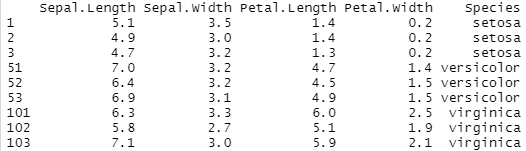
\includegraphics[width=5.95833in,height=\textheight]{Figure/ch2_ex_21_1.png}

\begin{itemize}
\item
  \texttt{iris}의 변수 \texttt{Sepal.Length}, \texttt{Sepal.Width}, \texttt{Petal.Length}, \texttt{Petal.Width}에는 꽃잎과 꽃받침의 길이와 폭을 측정한 결과가 입력되어 있다. 세 가지 붓꽃 종류별로 네 변수의 평균값을 각각 계산해 보자
\item
  150송이 중 \texttt{Petal.Width}의 값이 1 이하이고 \texttt{Petal.Length}가 4 이하인 붓꽃이 모두 몇 송이가 있는지 알아보자. 또한 세 종류의 붓꽃별로는 각각 몇 송이가 있는지 알아보자.
\end{itemize}

\begin{enumerate}
\def\labelenumi{\arabic{enumi}.}
\setcounter{enumi}{1}
\tightlist
\item
  데이터 프레임 \texttt{mtcars}는 1974년에 발행된 어떤 잡지에 소개된 32대 자동차의 연비와 관련된 자료이다.
\end{enumerate}

\begin{itemize}
\tightlist
\item
  숫자형 변수 \texttt{mpg}에 대한 다음의 조건으로 요인 \texttt{grade}를 생성해 보자. 단, \(\bar{x}\)와 \(sd\)는 변수 \texttt{mpg}의 평균 및 표준편차이다.
\end{itemize}

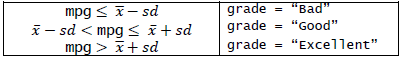
\includegraphics{Figure/ch2_ex_21_2.PNG}

\begin{itemize}
\item
  \texttt{mtcars}의 행 이름을 데이터 프레임에 변수 이름 \texttt{model}로 추가해 보자
\item
  요인 \texttt{grade}가 \texttt{Excellent}인 자동차의 변수 \texttt{model}과 \texttt{mpg}의 값을 출력해 보자.
\item
  요인 \texttt{grade}가 \texttt{Bad}인 자동차들의 평균 \texttt{mpg} 값을 계산해 보자.
\end{itemize}

\hypertarget{uxb370uxc774uxd130-uxc785uxb825}{%
\chapter{데이터 입력}\label{uxb370uxc774uxd130-uxc785uxb825}}

Placeholder

\hypertarget{uxd14duxc2a4uxd2b8-uxd30cuxc77c-uxbd88uxb7ecuxc624uxae30-uxd328uxd0a4uxc9c0-readr-uxd568uxc218uxc758-uxd65cuxc6a9}{%
\section{\texorpdfstring{텍스트 파일 불러오기: 패키지 \texttt{readr} 함수의 활용}{텍스트 파일 불러오기: 패키지 readr 함수의 활용}}\label{uxd14duxc2a4uxd2b8-uxd30cuxc77c-uxbd88uxb7ecuxc624uxae30-uxd328uxd0a4uxc9c0-readr-uxd568uxc218uxc758-uxd65cuxc6a9}}

\hypertarget{uxd568uxc218-read_tableuxb85c-uxb370uxc774uxd130-uxd30cuxc77c-uxbd88uxb7ecuxc624uxae30}{%
\subsection{\texorpdfstring{함수 \texttt{read\_table()}로 데이터 파일 불러오기}{함수 read\_table()로 데이터 파일 불러오기}}\label{uxd568uxc218-read_tableuxb85c-uxb370uxc774uxd130-uxd30cuxc77c-uxbd88uxb7ecuxc624uxae30}}

\hypertarget{uxd568uxc218-read_csvuxb85c-csv-uxb370uxc774uxd130-uxd30cuxc77c-uxbd88uxb7ecuxc624uxae30}{%
\subsection{\texorpdfstring{함수 \texttt{read\_csv()}로 CSV 데이터 파일 불러오기}{함수 read\_csv()로 CSV 데이터 파일 불러오기}}\label{uxd568uxc218-read_csvuxb85c-csv-uxb370uxc774uxd130-uxd30cuxc77c-uxbd88uxb7ecuxc624uxae30}}

\hypertarget{uxd568uxc218-read_fwfuxb85c-uxace0uxc815-uxd3ecuxb9f7-uxad6cuxc870uxb97c-uxac16uxb294-uxb370uxc774uxd130-uxd30cuxc77c-uxbd88uxb7ecuxc624uxae30}{%
\subsection{\texorpdfstring{함수 \texttt{read\_fwf()}로 고정 포맷 구조를 갖는 데이터 파일 불러오기}{함수 read\_fwf()로 고정 포맷 구조를 갖는 데이터 파일 불러오기}}\label{uxd568uxc218-read_fwfuxb85c-uxace0uxc815-uxd3ecuxb9f7-uxad6cuxc870uxb97c-uxac16uxb294-uxb370uxc774uxd130-uxd30cuxc77c-uxbd88uxb7ecuxc624uxae30}}

\hypertarget{excel-uxd30cuxc77c-uxbd88uxb7ecuxc624uxae30}{%
\section{Excel 파일 불러오기}\label{excel-uxd30cuxc77c-uxbd88uxb7ecuxc624uxae30}}

\hypertarget{sas-uxb370uxc774uxd130-uxd30cuxc77c-uxbd88uxb7ecuxc624uxae30}{%
\section{SAS 데이터 파일 불러오기}\label{sas-uxb370uxc774uxd130-uxd30cuxc77c-uxbd88uxb7ecuxc624uxae30}}

\hypertarget{html-uxd14cuxc774uxbe14-uxbd88uxb7ecuxc624uxae30}{%
\section{HTML 테이블 불러오기}\label{html-uxd14cuxc774uxbe14-uxbd88uxb7ecuxc624uxae30}}

\hypertarget{dplyruxc5d0-uxc758uxd55c-uxb370uxc774uxd130-uxb2e4uxb4ecuxae30}{%
\chapter{\texorpdfstring{\texttt{dplyr}에 의한 데이터 다듬기}{dplyr에 의한 데이터 다듬기}}\label{dplyruxc5d0-uxc758uxd55c-uxb370uxc774uxd130-uxb2e4uxb4ecuxae30}}

Placeholder

\hypertarget{uxd589uxc744-uxc791uxc5c5-uxb300uxc0c1uxc73cuxb85c-uxd558uxb294-uxd568uxc218}{%
\section{행을 작업 대상으로 하는 함수}\label{uxd589uxc744-uxc791uxc5c5-uxb300uxc0c1uxc73cuxb85c-uxd558uxb294-uxd568uxc218}}

\hypertarget{uxc870uxac74uxc5d0-uxc758uxd55c-uxd589-uxc120uxd0dd-filter}{%
\subsection{\texorpdfstring{조건에 의한 행 선택: \texttt{filter()}}{조건에 의한 행 선택: filter()}}\label{uxc870uxac74uxc5d0-uxc758uxd55c-uxd589-uxc120uxd0dd-filter}}

\hypertarget{uxc704uxce58uxc5d0-uxc758uxd55c-uxd589-uxc120uxd0dd-slice-uxbc0f-uxadf8uxc640-uxad00uxb828uxb41c-uxd568uxc218}{%
\subsection{\texorpdfstring{위치에 의한 행 선택: \texttt{slice()} 및 그와 관련된 함수}{위치에 의한 행 선택: slice() 및 그와 관련된 함수}}\label{uxc704uxce58uxc5d0-uxc758uxd55c-uxd589-uxc120uxd0dd-slice-uxbc0f-uxadf8uxc640-uxad00uxb828uxb41c-uxd568uxc218}}

\hypertarget{uxd589uxc758-uxc815uxb82c-arrange}{%
\subsection{\texorpdfstring{행의 정렬: \texttt{arrange()}}{행의 정렬: arrange()}}\label{uxd589uxc758-uxc815uxb82c-arrange}}

\hypertarget{uxc911uxbcf5uxb41c-uxd589uxc758-uxc81cuxac70-distinct}{%
\subsection{\texorpdfstring{중복된 행의 제거: \texttt{distinct()}}{중복된 행의 제거: distinct()}}\label{uxc911uxbcf5uxb41c-uxd589uxc758-uxc81cuxac70-distinct}}

\hypertarget{uxc5f4uxc744-uxc791uxc5c5-uxb300uxc0c1uxc73cuxb85c-uxd558uxb294-uxd568uxc218}{%
\section{열을 작업 대상으로 하는 함수}\label{uxc5f4uxc744-uxc791uxc5c5-uxb300uxc0c1uxc73cuxb85c-uxd558uxb294-uxd568uxc218}}

\hypertarget{uxc5f4uxc758-uxc120uxd0dd-select}{%
\subsection{\texorpdfstring{열의 선택: \texttt{select()}}{열의 선택: select()}}\label{uxc5f4uxc758-uxc120uxd0dd-select}}

\hypertarget{uxc5f4-uxc774uxb984-uxbcc0uxacbd-renameuxacfc-rename_with}{%
\subsection{\texorpdfstring{열 이름 변경: \texttt{rename()}과 \texttt{rename\_with()}}{열 이름 변경: rename()과 rename\_with()}}\label{uxc5f4-uxc774uxb984-uxbcc0uxacbd-renameuxacfc-rename_with}}

\hypertarget{uxc5f4uxc758-uxc704uxce58-uxbcc0uxacbd-relocate}{%
\subsection{\texorpdfstring{열의 위치 변경: \texttt{relocate()}}{열의 위치 변경: relocate()}}\label{uxc5f4uxc758-uxc704uxce58-uxbcc0uxacbd-relocate}}

\hypertarget{uxc0c8uxb85cuxc6b4-uxc5f4uxc758-uxcd94uxac00-mutateuxc640-transmute}{%
\subsection{\texorpdfstring{새로운 열의 추가: \texttt{mutate()}와 \texttt{transmute()}}{새로운 열의 추가: mutate()와 transmute()}}\label{uxc0c8uxb85cuxc6b4-uxc5f4uxc758-uxcd94uxac00-mutateuxc640-transmute}}

\hypertarget{uxc5ecuxb7ec-uxd589-uxc790uxb8ccuxc758-uxc694uxc57d-summarise}{%
\section{\texorpdfstring{여러 행 자료의 요약: \texttt{summarise()}}{여러 행 자료의 요약: summarise()}}\label{uxc5ecuxb7ec-uxd589-uxc790uxb8ccuxc758-uxc694uxc57d-summarise}}

  \bibliography{book.bib,packages.bib}

\end{document}
